\documentclass[twoside]{book}

% Packages required by doxygen
\usepackage{fixltx2e}
\usepackage{calc}
\usepackage{doxygen}
\usepackage[export]{adjustbox} % also loads graphicx
\usepackage{graphicx}
\usepackage[utf8]{inputenc}
\usepackage{makeidx}
\usepackage{multicol}
\usepackage{multirow}
\PassOptionsToPackage{warn}{textcomp}
\usepackage{textcomp}
\usepackage[nointegrals]{wasysym}
\usepackage[table]{xcolor}

% Font selection
\usepackage[T1]{fontenc}
\usepackage[scaled=.90]{helvet}
\usepackage{courier}
\usepackage{amssymb}
\usepackage{sectsty}
\renewcommand{\familydefault}{\sfdefault}
\allsectionsfont{%
  \fontseries{bc}\selectfont%
  \color{darkgray}%
}
\renewcommand{\DoxyLabelFont}{%
  \fontseries{bc}\selectfont%
  \color{darkgray}%
}
\newcommand{\+}{\discretionary{\mbox{\scriptsize$\hookleftarrow$}}{}{}}

% Page & text layout
\usepackage{geometry}
\geometry{%
  a4paper,%
  top=2.5cm,%
  bottom=2.5cm,%
  left=2.5cm,%
  right=2.5cm%
}
\tolerance=750
\hfuzz=15pt
\hbadness=750
\setlength{\emergencystretch}{15pt}
\setlength{\parindent}{0cm}
\setlength{\parskip}{3ex plus 2ex minus 2ex}
\makeatletter
\renewcommand{\paragraph}{%
  \@startsection{paragraph}{4}{0ex}{-1.0ex}{1.0ex}{%
    \normalfont\normalsize\bfseries\SS@parafont%
  }%
}
\renewcommand{\subparagraph}{%
  \@startsection{subparagraph}{5}{0ex}{-1.0ex}{1.0ex}{%
    \normalfont\normalsize\bfseries\SS@subparafont%
  }%
}
\makeatother

% Headers & footers
\usepackage{fancyhdr}
\pagestyle{fancyplain}
\fancyhead[LE]{\fancyplain{}{\bfseries\thepage}}
\fancyhead[CE]{\fancyplain{}{}}
\fancyhead[RE]{\fancyplain{}{\bfseries\leftmark}}
\fancyhead[LO]{\fancyplain{}{\bfseries\rightmark}}
\fancyhead[CO]{\fancyplain{}{}}
\fancyhead[RO]{\fancyplain{}{\bfseries\thepage}}
\fancyfoot[LE]{\fancyplain{}{}}
\fancyfoot[CE]{\fancyplain{}{}}
\fancyfoot[RE]{\fancyplain{}{\bfseries\scriptsize Generated by Doxygen }}
\fancyfoot[LO]{\fancyplain{}{\bfseries\scriptsize Generated by Doxygen }}
\fancyfoot[CO]{\fancyplain{}{}}
\fancyfoot[RO]{\fancyplain{}{}}
\renewcommand{\footrulewidth}{0.4pt}
\renewcommand{\chaptermark}[1]{%
  \markboth{#1}{}%
}
\renewcommand{\sectionmark}[1]{%
  \markright{\thesection\ #1}%
}

% Indices & bibliography
\usepackage{natbib}
\usepackage[titles]{tocloft}
\setcounter{tocdepth}{3}
\setcounter{secnumdepth}{5}
\makeindex

% Hyperlinks (required, but should be loaded last)
\usepackage{ifpdf}
\ifpdf
  \usepackage[pdftex,pagebackref=true]{hyperref}
\else
  \usepackage[ps2pdf,pagebackref=true]{hyperref}
\fi
\hypersetup{%
  colorlinks=true,%
  linkcolor=blue,%
  citecolor=blue,%
  unicode%
}

% Custom commands
\newcommand{\clearemptydoublepage}{%
  \newpage{\pagestyle{empty}\cleardoublepage}%
}

\usepackage{caption}
\captionsetup{labelsep=space,justification=centering,font={bf},singlelinecheck=off,skip=4pt,position=top}

%===== C O N T E N T S =====

\begin{document}

% Titlepage & ToC
\hypersetup{pageanchor=false,
             bookmarksnumbered=true,
             pdfencoding=unicode
            }
\pagenumbering{roman}
\begin{titlepage}
\vspace*{7cm}
\begin{center}%
{\Large Final Assignment \\[1ex]\large 1.\+0 }\\
\vspace*{1cm}
{\large Generated by Doxygen 1.8.11}\\
\end{center}
\end{titlepage}
\clearemptydoublepage
\tableofcontents
\clearemptydoublepage
\pagenumbering{arabic}
\hypersetup{pageanchor=true}

%--- Begin generated contents ---
\chapter{Project Description}
\label{index}\hypertarget{index}{}This code was developed for final assignment of the experimental course. Please read the readme file contined in the following git repository\+: \href{https://github.com/FraTesta/experimental_ws.git}{\tt https\+://github.\+com/\+Fra\+Testa/experimental\+\_\+ws.\+git} 
\chapter{doc}
\label{md_doc_pages_doc}
\hypertarget{md_doc_pages_doc}{}
\input{md_doc_pages_doc}
\chapter{Namespace Index}
\section{Packages}
Here are the packages with brief descriptions (if available)\+:\begin{DoxyCompactList}
\item\contentsline{section}{\hyperlink{namespacecommandManager}{command\+Manager} }{\pageref{namespacecommandManager}}{}
\item\contentsline{section}{\hyperlink{namespacenoSleep}{no\+Sleep} }{\pageref{namespacenoSleep}}{}
\item\contentsline{section}{\hyperlink{namespaceroomDetector}{room\+Detector} }{\pageref{namespaceroomDetector}}{}
\item\contentsline{section}{\hyperlink{namespaceRooms}{Rooms} }{\pageref{namespaceRooms}}{}
\item\contentsline{section}{\hyperlink{namespacetrack}{track} }{\pageref{namespacetrack}}{}
\item\contentsline{section}{\hyperlink{namespaceUI}{UI} }{\pageref{namespaceUI}}{}
\end{DoxyCompactList}

\chapter{Hierarchical Index}
\section{Class Hierarchy}
This inheritance list is sorted roughly, but not completely, alphabetically\+:\begin{DoxyCompactList}
\item State\begin{DoxyCompactList}
\item \contentsline{section}{F\+S\+M.\+Normal}{\pageref{classFSM_1_1Normal}}{}
\item \contentsline{section}{F\+S\+M.\+Play}{\pageref{classFSM_1_1Play}}{}
\item \contentsline{section}{F\+S\+M.\+Sleep}{\pageref{classFSM_1_1Sleep}}{}
\item \contentsline{section}{F\+S\+Mplay.\+Normal}{\pageref{classFSMplay_1_1Normal}}{}
\item \contentsline{section}{F\+S\+Mplay.\+Play}{\pageref{classFSMplay_1_1Play}}{}
\item \contentsline{section}{F\+S\+Mplay.\+Sleep}{\pageref{classFSMplay_1_1Sleep}}{}
\item \contentsline{section}{state\+\_\+machine.\+Locked}{\pageref{classstate__machine_1_1Locked}}{}
\item \contentsline{section}{state\+\_\+machine.\+Unlocked}{\pageref{classstate__machine_1_1Unlocked}}{}
\end{DoxyCompactList}
\end{DoxyCompactList}

\chapter{Class Index}
\section{Class List}
Here are the classes, structs, unions and interfaces with brief descriptions\+:\begin{DoxyCompactList}
\item\contentsline{section}{\hyperlink{classcm2_1_1Find}{cm2.\+Find} }{\pageref{classcm2_1_1Find}}{}
\item\contentsline{section}{\hyperlink{classcommandManager_1_1Find}{command\+Manager.\+Find} }{\pageref{classcommandManager_1_1Find}}{}
\item\contentsline{section}{\hyperlink{classtimerProva_1_1lol}{timer\+Prova.\+lol} }{\pageref{classtimerProva_1_1lol}}{}
\item\contentsline{section}{\hyperlink{classcm2_1_1Normal}{cm2.\+Normal} }{\pageref{classcm2_1_1Normal}}{}
\item\contentsline{section}{\hyperlink{classcommandManager_1_1Normal}{command\+Manager.\+Normal} }{\pageref{classcommandManager_1_1Normal}}{}
\item\contentsline{section}{\hyperlink{classcommandManager_1_1Play}{command\+Manager.\+Play} }{\pageref{classcommandManager_1_1Play}}{}
\item\contentsline{section}{\hyperlink{classcm2_1_1Play}{cm2.\+Play} }{\pageref{classcm2_1_1Play}}{}
\item\contentsline{section}{\hyperlink{classroomDetector_1_1roomDetector}{room\+Detector.\+room\+Detector} \\*This class implements a subscriber to the camera topic of the robot and applies several open\+CV mask in order to recognise the color of the ball, then it send the detected color to the \hyperlink{namespacecommandManager}{command\+Manager} node }{\pageref{classroomDetector_1_1roomDetector}}{}
\item\contentsline{section}{\hyperlink{classroomsDetection_1_1roomDetector}{rooms\+Detection.\+room\+Detector} }{\pageref{classroomsDetection_1_1roomDetector}}{}
\item\contentsline{section}{\hyperlink{classRooms_1_1Rooms}{Rooms.\+Rooms} }{\pageref{classRooms_1_1Rooms}}{}
\item\contentsline{section}{\hyperlink{classcm2_1_1Sleep}{cm2.\+Sleep} }{\pageref{classcm2_1_1Sleep}}{}
\item\contentsline{section}{\hyperlink{classcommandManager_1_1Sleep}{command\+Manager.\+Sleep} }{\pageref{classcommandManager_1_1Sleep}}{}
\item\contentsline{section}{\hyperlink{classcommandManager_1_1Track}{command\+Manager.\+Track} }{\pageref{classcommandManager_1_1Track}}{}
\item\contentsline{section}{\hyperlink{classcm2_1_1Track}{cm2.\+Track} }{\pageref{classcm2_1_1Track}}{}
\item\contentsline{section}{\hyperlink{classtrackObj_1_1TrackAction}{track\+Obj.\+Track\+Action} \\*Class that implements the action server for tracking the ball }{\pageref{classtrackObj_1_1TrackAction}}{}
\item\contentsline{section}{\hyperlink{classtrack_1_1TrackAction}{track.\+Track\+Action} \\*Class that implements the action server for tracking the ball }{\pageref{classtrack_1_1TrackAction}}{}
\end{DoxyCompactList}

\chapter{File Index}
\section{File List}
Here is a list of all files with brief descriptions\+:\begin{DoxyCompactList}
\item\contentsline{section}{/home/experimental\+\_\+ws/src/final\+\_\+assignment/scripts/\hyperlink{cm2_8py}{cm2.\+py} }{\pageref{cm2_8py}}{}
\item\contentsline{section}{/home/experimental\+\_\+ws/src/final\+\_\+assignment/scripts/\hyperlink{cmd__smach_8py}{cmd\+\_\+smach.\+py} }{\pageref{cmd__smach_8py}}{}
\item\contentsline{section}{/home/experimental\+\_\+ws/src/final\+\_\+assignment/scripts/\hyperlink{commandManager_8py}{command\+Manager.\+py} \\*This script is a node which is the core of the entier project }{\pageref{commandManager_8py}}{}
\item\contentsline{section}{/home/experimental\+\_\+ws/src/final\+\_\+assignment/scripts/\hyperlink{roomDetector_8py}{room\+Detector.\+py} \\*This script implements the \hyperlink{namespaceroomDetector}{room\+Detector} class which basically is able to detect a ball and publish its color on the new\+Room topic }{\pageref{roomDetector_8py}}{}
\item\contentsline{section}{/home/experimental\+\_\+ws/src/final\+\_\+assignment/scripts/\hyperlink{Rooms_8py}{Rooms.\+py} \\*This script contains the \hyperlink{namespaceRooms}{Rooms} class, which implements a structure dedicated to the control and management of the rooms in a given environment }{\pageref{Rooms_8py}}{}
\item\contentsline{section}{/home/experimental\+\_\+ws/src/final\+\_\+assignment/scripts/\hyperlink{roomsDetection_8py}{rooms\+Detection.\+py} }{\pageref{roomsDetection_8py}}{}
\item\contentsline{section}{/home/experimental\+\_\+ws/src/final\+\_\+assignment/scripts/\hyperlink{timerProva_8py}{timer\+Prova.\+py} }{\pageref{timerProva_8py}}{}
\item\contentsline{section}{/home/experimental\+\_\+ws/src/final\+\_\+assignment/scripts/\hyperlink{track_8py}{track.\+py} \\*This script is an acttion server which takes a color of a ball in proximity of the robot and start to track it }{\pageref{track_8py}}{}
\item\contentsline{section}{/home/experimental\+\_\+ws/src/final\+\_\+assignment/scripts/\hyperlink{UI_8py}{U\+I.\+py} }{\pageref{UI_8py}}{}
\end{DoxyCompactList}

\chapter{Namespace Documentation}
\hypertarget{namespacecommandManager}{}\section{command\+Manager Namespace Reference}
\label{namespacecommandManager}\index{command\+Manager@{command\+Manager}}
\subsection*{Classes}
\begin{DoxyCompactItemize}
\item 
class \hyperlink{classcommandManager_1_1Find}{Find}
\item 
class \hyperlink{classcommandManager_1_1Normal}{Normal}
\item 
class \hyperlink{classcommandManager_1_1Play}{Play}
\item 
class \hyperlink{classcommandManager_1_1Sleep}{Sleep}
\item 
class \hyperlink{classcommandManager_1_1Track}{Track}
\end{DoxyCompactItemize}
\subsection*{Functions}
\begin{DoxyCompactItemize}
\item 
def \hyperlink{namespacecommandManager_a2310383d56755f0a09a75b1a92130e21}{U\+Icallback} (data)
\item 
def \hyperlink{namespacecommandManager_aa96fd2ed94c8c1168e09ced4015dcb1b}{new\+Room\+Detected} (color)
\item 
def \hyperlink{namespacecommandManager_af8e54858c65310eb1e131529bf200516}{move\+\_\+base\+\_\+go\+\_\+to} (x, y)
\item 
def \hyperlink{namespacecommandManager_ae8b570eb4bf393859bc74c9cb5fe125f}{main} ()
\end{DoxyCompactItemize}
\subsection*{Variables}
\begin{DoxyCompactItemize}
\item 
bool \hyperlink{namespacecommandManager_aecd980edd677f32e8693cbd21fa2c6eb}{P\+L\+AY} = False
\begin{DoxyCompactList}\small\item\em Flag which notify when the user types \textquotesingle{}play\textquotesingle{}. \end{DoxyCompactList}\item 
string \hyperlink{namespacecommandManager_ace76b1a89b584c851c50bc3ad66e1d69}{T\+A\+R\+G\+E\+T\+\_\+\+R\+O\+OM} = \char`\"{}None\char`\"{}
\begin{DoxyCompactList}\small\item\em Contains the desired room entered by the user. \end{DoxyCompactList}\item 
bool \hyperlink{namespacecommandManager_a6356544112d78464670ffb9af59bed1d}{N\+E\+W\+\_\+\+TR} = False
\begin{DoxyCompactList}\small\item\em Flag which notify when the command manager recives a new target room. \end{DoxyCompactList}\item 
bool \hyperlink{namespacecommandManager_a52e7163bf2cde17330107e6a2cf2f851}{N\+E\+W\+\_\+\+R\+O\+OM} = False
\begin{DoxyCompactList}\small\item\em new room detected \end{DoxyCompactList}\item 
bool \hyperlink{namespacecommandManager_afb1c5b8d9e6c746c82f4abf3fffe02a5}{R\+A\+N\+D\+OM} = True
\begin{DoxyCompactList}\small\item\em Random position generation flag. \end{DoxyCompactList}\item 
string \hyperlink{namespacecommandManager_ae945cfc4fe1632a6952debd7a67d9f3c}{C\+O\+L\+O\+R\+\_\+\+R\+O\+OM} = \char`\"{}None\char`\"{}
\begin{DoxyCompactList}\small\item\em color of the detected ball \end{DoxyCompactList}\item 
bool \hyperlink{namespacecommandManager_ad0728881cc70cfd3f8f5251b7b9af646}{F\+I\+N\+D\+\_\+\+M\+O\+DE} = False
\begin{DoxyCompactList}\small\item\em Flag to comeback into \hyperlink{classcommandManager_1_1Find}{Find} state when it\textquotesingle{}s necessary. \end{DoxyCompactList}\item 
\hyperlink{namespacecommandManager_ad81f5cdd9bf18b67989c77a2329b9e28}{client} = actionlib.\+Simple\+Action\+Client(\textquotesingle{}move\+\_\+base\textquotesingle{},Move\+Base\+Action)
\begin{DoxyCompactList}\small\item\em init the move\+\_\+base client \end{DoxyCompactList}\item 
\hyperlink{namespacecommandManager_a868809e1f6a79e7b7ce5ea405e978d48}{rooms} = \hyperlink{classRooms_1_1Rooms}{Rooms}()
\begin{DoxyCompactList}\small\item\em init the rooms environment \end{DoxyCompactList}\end{DoxyCompactItemize}


\subsection{Function Documentation}
\index{command\+Manager@{command\+Manager}!main@{main}}
\index{main@{main}!command\+Manager@{command\+Manager}}
\subsubsection[{\texorpdfstring{main()}{main()}}]{\setlength{\rightskip}{0pt plus 5cm}def command\+Manager.\+main (
\begin{DoxyParamCaption}
{}
\end{DoxyParamCaption}
)}\hypertarget{namespacecommandManager_ae8b570eb4bf393859bc74c9cb5fe125f}{}\label{namespacecommandManager_ae8b570eb4bf393859bc74c9cb5fe125f}
\index{command\+Manager@{command\+Manager}!move\+\_\+base\+\_\+go\+\_\+to@{move\+\_\+base\+\_\+go\+\_\+to}}
\index{move\+\_\+base\+\_\+go\+\_\+to@{move\+\_\+base\+\_\+go\+\_\+to}!command\+Manager@{command\+Manager}}
\subsubsection[{\texorpdfstring{move\+\_\+base\+\_\+go\+\_\+to(x, y)}{move_base_go_to(x, y)}}]{\setlength{\rightskip}{0pt plus 5cm}def command\+Manager.\+move\+\_\+base\+\_\+go\+\_\+to (
\begin{DoxyParamCaption}
\item[{}]{x, }
\item[{}]{y}
\end{DoxyParamCaption}
)}\hypertarget{namespacecommandManager_af8e54858c65310eb1e131529bf200516}{}\label{namespacecommandManager_af8e54858c65310eb1e131529bf200516}
\index{command\+Manager@{command\+Manager}!new\+Room\+Detected@{new\+Room\+Detected}}
\index{new\+Room\+Detected@{new\+Room\+Detected}!command\+Manager@{command\+Manager}}
\subsubsection[{\texorpdfstring{new\+Room\+Detected(color)}{newRoomDetected(color)}}]{\setlength{\rightskip}{0pt plus 5cm}def command\+Manager.\+new\+Room\+Detected (
\begin{DoxyParamCaption}
\item[{}]{color}
\end{DoxyParamCaption}
)}\hypertarget{namespacecommandManager_aa96fd2ed94c8c1168e09ced4015dcb1b}{}\label{namespacecommandManager_aa96fd2ed94c8c1168e09ced4015dcb1b}
\index{command\+Manager@{command\+Manager}!U\+Icallback@{U\+Icallback}}
\index{U\+Icallback@{U\+Icallback}!command\+Manager@{command\+Manager}}
\subsubsection[{\texorpdfstring{U\+Icallback(data)}{UIcallback(data)}}]{\setlength{\rightskip}{0pt plus 5cm}def command\+Manager.\+U\+Icallback (
\begin{DoxyParamCaption}
\item[{}]{data}
\end{DoxyParamCaption}
)}\hypertarget{namespacecommandManager_a2310383d56755f0a09a75b1a92130e21}{}\label{namespacecommandManager_a2310383d56755f0a09a75b1a92130e21}


\subsection{Variable Documentation}
\index{command\+Manager@{command\+Manager}!client@{client}}
\index{client@{client}!command\+Manager@{command\+Manager}}
\subsubsection[{\texorpdfstring{client}{client}}]{\setlength{\rightskip}{0pt plus 5cm}command\+Manager.\+client = actionlib.\+Simple\+Action\+Client(\textquotesingle{}move\+\_\+base\textquotesingle{},Move\+Base\+Action)}\hypertarget{namespacecommandManager_ad81f5cdd9bf18b67989c77a2329b9e28}{}\label{namespacecommandManager_ad81f5cdd9bf18b67989c77a2329b9e28}


init the move\+\_\+base client 

\index{command\+Manager@{command\+Manager}!C\+O\+L\+O\+R\+\_\+\+R\+O\+OM@{C\+O\+L\+O\+R\+\_\+\+R\+O\+OM}}
\index{C\+O\+L\+O\+R\+\_\+\+R\+O\+OM@{C\+O\+L\+O\+R\+\_\+\+R\+O\+OM}!command\+Manager@{command\+Manager}}
\subsubsection[{\texorpdfstring{C\+O\+L\+O\+R\+\_\+\+R\+O\+OM}{COLOR_ROOM}}]{\setlength{\rightskip}{0pt plus 5cm}string command\+Manager.\+C\+O\+L\+O\+R\+\_\+\+R\+O\+OM = \char`\"{}None\char`\"{}}\hypertarget{namespacecommandManager_ae945cfc4fe1632a6952debd7a67d9f3c}{}\label{namespacecommandManager_ae945cfc4fe1632a6952debd7a67d9f3c}


color of the detected ball 

\index{command\+Manager@{command\+Manager}!F\+I\+N\+D\+\_\+\+M\+O\+DE@{F\+I\+N\+D\+\_\+\+M\+O\+DE}}
\index{F\+I\+N\+D\+\_\+\+M\+O\+DE@{F\+I\+N\+D\+\_\+\+M\+O\+DE}!command\+Manager@{command\+Manager}}
\subsubsection[{\texorpdfstring{F\+I\+N\+D\+\_\+\+M\+O\+DE}{FIND_MODE}}]{\setlength{\rightskip}{0pt plus 5cm}bool command\+Manager.\+F\+I\+N\+D\+\_\+\+M\+O\+DE = False}\hypertarget{namespacecommandManager_ad0728881cc70cfd3f8f5251b7b9af646}{}\label{namespacecommandManager_ad0728881cc70cfd3f8f5251b7b9af646}


Flag to comeback into \hyperlink{classcommandManager_1_1Find}{Find} state when it\textquotesingle{}s necessary. 

\index{command\+Manager@{command\+Manager}!N\+E\+W\+\_\+\+R\+O\+OM@{N\+E\+W\+\_\+\+R\+O\+OM}}
\index{N\+E\+W\+\_\+\+R\+O\+OM@{N\+E\+W\+\_\+\+R\+O\+OM}!command\+Manager@{command\+Manager}}
\subsubsection[{\texorpdfstring{N\+E\+W\+\_\+\+R\+O\+OM}{NEW_ROOM}}]{\setlength{\rightskip}{0pt plus 5cm}bool command\+Manager.\+N\+E\+W\+\_\+\+R\+O\+OM = False}\hypertarget{namespacecommandManager_a52e7163bf2cde17330107e6a2cf2f851}{}\label{namespacecommandManager_a52e7163bf2cde17330107e6a2cf2f851}


new room detected 

\index{command\+Manager@{command\+Manager}!N\+E\+W\+\_\+\+TR@{N\+E\+W\+\_\+\+TR}}
\index{N\+E\+W\+\_\+\+TR@{N\+E\+W\+\_\+\+TR}!command\+Manager@{command\+Manager}}
\subsubsection[{\texorpdfstring{N\+E\+W\+\_\+\+TR}{NEW_TR}}]{\setlength{\rightskip}{0pt plus 5cm}bool command\+Manager.\+N\+E\+W\+\_\+\+TR = False}\hypertarget{namespacecommandManager_a6356544112d78464670ffb9af59bed1d}{}\label{namespacecommandManager_a6356544112d78464670ffb9af59bed1d}


Flag which notify when the command manager recives a new target room. 

\index{command\+Manager@{command\+Manager}!P\+L\+AY@{P\+L\+AY}}
\index{P\+L\+AY@{P\+L\+AY}!command\+Manager@{command\+Manager}}
\subsubsection[{\texorpdfstring{P\+L\+AY}{PLAY}}]{\setlength{\rightskip}{0pt plus 5cm}bool command\+Manager.\+P\+L\+AY = False}\hypertarget{namespacecommandManager_aecd980edd677f32e8693cbd21fa2c6eb}{}\label{namespacecommandManager_aecd980edd677f32e8693cbd21fa2c6eb}


Flag which notify when the user types \textquotesingle{}play\textquotesingle{}. 

\index{command\+Manager@{command\+Manager}!R\+A\+N\+D\+OM@{R\+A\+N\+D\+OM}}
\index{R\+A\+N\+D\+OM@{R\+A\+N\+D\+OM}!command\+Manager@{command\+Manager}}
\subsubsection[{\texorpdfstring{R\+A\+N\+D\+OM}{RANDOM}}]{\setlength{\rightskip}{0pt plus 5cm}bool command\+Manager.\+R\+A\+N\+D\+OM = True}\hypertarget{namespacecommandManager_afb1c5b8d9e6c746c82f4abf3fffe02a5}{}\label{namespacecommandManager_afb1c5b8d9e6c746c82f4abf3fffe02a5}


Random position generation flag. 

\index{command\+Manager@{command\+Manager}!rooms@{rooms}}
\index{rooms@{rooms}!command\+Manager@{command\+Manager}}
\subsubsection[{\texorpdfstring{rooms}{rooms}}]{\setlength{\rightskip}{0pt plus 5cm}command\+Manager.\+rooms = {\bf Rooms}()}\hypertarget{namespacecommandManager_a868809e1f6a79e7b7ce5ea405e978d48}{}\label{namespacecommandManager_a868809e1f6a79e7b7ce5ea405e978d48}


init the rooms environment 

\index{command\+Manager@{command\+Manager}!T\+A\+R\+G\+E\+T\+\_\+\+R\+O\+OM@{T\+A\+R\+G\+E\+T\+\_\+\+R\+O\+OM}}
\index{T\+A\+R\+G\+E\+T\+\_\+\+R\+O\+OM@{T\+A\+R\+G\+E\+T\+\_\+\+R\+O\+OM}!command\+Manager@{command\+Manager}}
\subsubsection[{\texorpdfstring{T\+A\+R\+G\+E\+T\+\_\+\+R\+O\+OM}{TARGET_ROOM}}]{\setlength{\rightskip}{0pt plus 5cm}string command\+Manager.\+T\+A\+R\+G\+E\+T\+\_\+\+R\+O\+OM = \char`\"{}None\char`\"{}}\hypertarget{namespacecommandManager_ace76b1a89b584c851c50bc3ad66e1d69}{}\label{namespacecommandManager_ace76b1a89b584c851c50bc3ad66e1d69}


Contains the desired room entered by the user. 


\hypertarget{namespacenoSleep}{}\section{no\+Sleep Namespace Reference}
\label{namespacenoSleep}\index{no\+Sleep@{no\+Sleep}}
\subsection*{Classes}
\begin{DoxyCompactItemize}
\item 
class \hyperlink{classnoSleep_1_1Find}{Find}
\item 
class \hyperlink{classnoSleep_1_1Normal}{Normal}
\item 
class \hyperlink{classnoSleep_1_1Play}{Play}
\item 
class \hyperlink{classnoSleep_1_1Sleep}{Sleep}
\item 
class \hyperlink{classnoSleep_1_1Track}{Track}
\end{DoxyCompactItemize}
\subsection*{Functions}
\begin{DoxyCompactItemize}
\item 
def \hyperlink{namespacenoSleep_a123223ff9a3dbafbd97e6d0f384396a2}{U\+Icallback} (data)
\begin{DoxyCompactList}\small\item\em Callback mathod of the U\+Isubscriber which handels the commands sent by the user. \end{DoxyCompactList}\item 
def \hyperlink{namespacenoSleep_afdab4949f2266a97c8e4f22565029431}{new\+Room\+Detected} (color)
\begin{DoxyCompactList}\small\item\em Callback function of the new\+Room\+Sub subscriber which recives the color of the new detected room. \end{DoxyCompactList}\item 
def \hyperlink{namespacenoSleep_a3f9d1f6206657669b0f1e0eb03e3faf8}{move\+\_\+base\+\_\+go\+\_\+to} (x, y)
\begin{DoxyCompactList}\small\item\em Method which prepares and send the goal to the move\+\_\+base action server. \end{DoxyCompactList}\item 
def \hyperlink{namespacenoSleep_a76829f5a5ea086115d4bbc161b5de95e}{main} ()
\end{DoxyCompactItemize}
\subsection*{Variables}
\begin{DoxyCompactItemize}
\item 
dictionary \hyperlink{namespacenoSleep_adbe81123b7abf75f19b461e802380fc1}{control\+\_\+variables}
\item 
\hyperlink{namespacenoSleep_ac8d2a8a17fd9bdac144f7cf8e268271d}{client} = actionlib.\+Simple\+Action\+Client(\textquotesingle{}move\+\_\+base\textquotesingle{},Move\+Base\+Action)
\begin{DoxyCompactList}\small\item\em Flag which notify when the user types \textquotesingle{}play\textquotesingle{} P\+L\+AY = False Contains the desired room entered by the user T\+A\+R\+G\+E\+T\+\_\+\+R\+O\+OM = \char`\"{}\+None\char`\"{} Flag which notify when the command manager recives a new target room from the user N\+E\+W\+\_\+\+TR = False Flag which notify that a new room was detected by the camera N\+E\+W\+\_\+\+R\+O\+OM = False Contains the color of the detected ball (room) N\+E\+W\+\_\+\+R\+O\+O\+M\+\_\+\+C\+O\+L\+OR = \char`\"{}\+None\char`\"{} Flag indicating if the F\+I\+ND mode is active or not F\+I\+N\+D\+\_\+\+M\+O\+DE = False Initialization of the move\+\_\+base client in order to assign target position to the move\+\_\+base action server. \end{DoxyCompactList}\item 
\hyperlink{namespacenoSleep_a9556e14c4f96e9bd3a98d6313f1c971b}{room\+D\+\_\+pub} = rospy.\+Publisher(\textquotesingle{}start\+RD\textquotesingle{}, Bool, queue\+\_\+size=10)
\begin{DoxyCompactList}\small\item\em Publisher to the start\+RD topic which allows to enable/disable the room detector. \end{DoxyCompactList}\item 
\hyperlink{namespacenoSleep_a5d68f48fa901f367ed63cd1e4ac1aef9}{rooms} = \hyperlink{classRooms_1_1Rooms}{Rooms}()
\begin{DoxyCompactList}\small\item\em Object of the class \hyperlink{namespaceRooms}{Rooms} necessary to store and manage the discovered rooms. \end{DoxyCompactList}\end{DoxyCompactItemize}


\subsection{Function Documentation}
\index{no\+Sleep@{no\+Sleep}!main@{main}}
\index{main@{main}!no\+Sleep@{no\+Sleep}}
\subsubsection[{\texorpdfstring{main()}{main()}}]{\setlength{\rightskip}{0pt plus 5cm}def no\+Sleep.\+main (
\begin{DoxyParamCaption}
{}
\end{DoxyParamCaption}
)}\hypertarget{namespacenoSleep_a76829f5a5ea086115d4bbc161b5de95e}{}\label{namespacenoSleep_a76829f5a5ea086115d4bbc161b5de95e}
\index{no\+Sleep@{no\+Sleep}!move\+\_\+base\+\_\+go\+\_\+to@{move\+\_\+base\+\_\+go\+\_\+to}}
\index{move\+\_\+base\+\_\+go\+\_\+to@{move\+\_\+base\+\_\+go\+\_\+to}!no\+Sleep@{no\+Sleep}}
\subsubsection[{\texorpdfstring{move\+\_\+base\+\_\+go\+\_\+to(x, y)}{move_base_go_to(x, y)}}]{\setlength{\rightskip}{0pt plus 5cm}def no\+Sleep.\+move\+\_\+base\+\_\+go\+\_\+to (
\begin{DoxyParamCaption}
\item[{}]{x, }
\item[{}]{y}
\end{DoxyParamCaption}
)}\hypertarget{namespacenoSleep_a3f9d1f6206657669b0f1e0eb03e3faf8}{}\label{namespacenoSleep_a3f9d1f6206657669b0f1e0eb03e3faf8}


Method which prepares and send the goal to the move\+\_\+base action server. 


\begin{DoxyParams}{Parameters}
{\em x} & X position of the desired goal \\
\hline
{\em y} & Y position of the desired goal \\
\hline
\end{DoxyParams}
\index{no\+Sleep@{no\+Sleep}!new\+Room\+Detected@{new\+Room\+Detected}}
\index{new\+Room\+Detected@{new\+Room\+Detected}!no\+Sleep@{no\+Sleep}}
\subsubsection[{\texorpdfstring{new\+Room\+Detected(color)}{newRoomDetected(color)}}]{\setlength{\rightskip}{0pt plus 5cm}def no\+Sleep.\+new\+Room\+Detected (
\begin{DoxyParamCaption}
\item[{}]{color}
\end{DoxyParamCaption}
)}\hypertarget{namespacenoSleep_afdab4949f2266a97c8e4f22565029431}{}\label{namespacenoSleep_afdab4949f2266a97c8e4f22565029431}


Callback function of the new\+Room\+Sub subscriber which recives the color of the new detected room. 


\begin{DoxyParams}{Parameters}
{\em color} & is a string message containing the color of the room detected by the \hyperlink{namespaceroomDetector}{room\+Detector} R\+OS node \\
\hline
\end{DoxyParams}
\index{no\+Sleep@{no\+Sleep}!U\+Icallback@{U\+Icallback}}
\index{U\+Icallback@{U\+Icallback}!no\+Sleep@{no\+Sleep}}
\subsubsection[{\texorpdfstring{U\+Icallback(data)}{UIcallback(data)}}]{\setlength{\rightskip}{0pt plus 5cm}def no\+Sleep.\+U\+Icallback (
\begin{DoxyParamCaption}
\item[{}]{data}
\end{DoxyParamCaption}
)}\hypertarget{namespacenoSleep_a123223ff9a3dbafbd97e6d0f384396a2}{}\label{namespacenoSleep_a123223ff9a3dbafbd97e6d0f384396a2}


Callback mathod of the U\+Isubscriber which handels the commands sent by the user. 


\begin{DoxyParams}{Parameters}
{\em data} & is a string message coming from the \hyperlink{namespaceUI}{UI} R\+OS node \\
\hline
\end{DoxyParams}


\subsection{Variable Documentation}
\index{no\+Sleep@{no\+Sleep}!client@{client}}
\index{client@{client}!no\+Sleep@{no\+Sleep}}
\subsubsection[{\texorpdfstring{client}{client}}]{\setlength{\rightskip}{0pt plus 5cm}no\+Sleep.\+client = actionlib.\+Simple\+Action\+Client(\textquotesingle{}move\+\_\+base\textquotesingle{},Move\+Base\+Action)}\hypertarget{namespacenoSleep_ac8d2a8a17fd9bdac144f7cf8e268271d}{}\label{namespacenoSleep_ac8d2a8a17fd9bdac144f7cf8e268271d}


Flag which notify when the user types \textquotesingle{}play\textquotesingle{} P\+L\+AY = False Contains the desired room entered by the user T\+A\+R\+G\+E\+T\+\_\+\+R\+O\+OM = \char`\"{}\+None\char`\"{} Flag which notify when the command manager recives a new target room from the user N\+E\+W\+\_\+\+TR = False Flag which notify that a new room was detected by the camera N\+E\+W\+\_\+\+R\+O\+OM = False Contains the color of the detected ball (room) N\+E\+W\+\_\+\+R\+O\+O\+M\+\_\+\+C\+O\+L\+OR = \char`\"{}\+None\char`\"{} Flag indicating if the F\+I\+ND mode is active or not F\+I\+N\+D\+\_\+\+M\+O\+DE = False Initialization of the move\+\_\+base client in order to assign target position to the move\+\_\+base action server. 

\index{no\+Sleep@{no\+Sleep}!control\+\_\+variables@{control\+\_\+variables}}
\index{control\+\_\+variables@{control\+\_\+variables}!no\+Sleep@{no\+Sleep}}
\subsubsection[{\texorpdfstring{control\+\_\+variables}{control_variables}}]{\setlength{\rightskip}{0pt plus 5cm}dictionary no\+Sleep.\+control\+\_\+variables}\hypertarget{namespacenoSleep_adbe81123b7abf75f19b461e802380fc1}{}\label{namespacenoSleep_adbe81123b7abf75f19b461e802380fc1}
{\bfseries Initial value\+:}
\begin{DoxyCode}
1 = \{
2     \textcolor{comment}{## Flag which notify when the user types 'play'}
3     \textcolor{stringliteral}{"PLAY"} : \textcolor{keyword}{False},
4     \textcolor{comment}{## Contains the desired room entered by the user }
5     \textcolor{stringliteral}{"TARGET\_ROOM"} : \textcolor{stringliteral}{"None"},
6     \textcolor{comment}{## Contains the color of the detected ball (room) }
7     \textcolor{stringliteral}{"NEW\_ROOM\_COLOR"} : \textcolor{stringliteral}{"None"},
8     \textcolor{comment}{## Flag indicating if the FIND mode is active or not }
9     \textcolor{stringliteral}{"FIND\_MODE"} : \textcolor{keyword}{False}   
10 \}
\end{DoxyCode}
\index{no\+Sleep@{no\+Sleep}!room\+D\+\_\+pub@{room\+D\+\_\+pub}}
\index{room\+D\+\_\+pub@{room\+D\+\_\+pub}!no\+Sleep@{no\+Sleep}}
\subsubsection[{\texorpdfstring{room\+D\+\_\+pub}{roomD_pub}}]{\setlength{\rightskip}{0pt plus 5cm}no\+Sleep.\+room\+D\+\_\+pub = rospy.\+Publisher(\textquotesingle{}start\+RD\textquotesingle{}, Bool, queue\+\_\+size=10)}\hypertarget{namespacenoSleep_a9556e14c4f96e9bd3a98d6313f1c971b}{}\label{namespacenoSleep_a9556e14c4f96e9bd3a98d6313f1c971b}


Publisher to the start\+RD topic which allows to enable/disable the room detector. 

\index{no\+Sleep@{no\+Sleep}!rooms@{rooms}}
\index{rooms@{rooms}!no\+Sleep@{no\+Sleep}}
\subsubsection[{\texorpdfstring{rooms}{rooms}}]{\setlength{\rightskip}{0pt plus 5cm}no\+Sleep.\+rooms = {\bf Rooms}()}\hypertarget{namespacenoSleep_a5d68f48fa901f367ed63cd1e4ac1aef9}{}\label{namespacenoSleep_a5d68f48fa901f367ed63cd1e4ac1aef9}


Object of the class \hyperlink{namespaceRooms}{Rooms} necessary to store and manage the discovered rooms. 


\hypertarget{namespaceroomDetector}{}\section{room\+Detector Namespace Reference}
\label{namespaceroomDetector}\index{room\+Detector@{room\+Detector}}
\subsection*{Classes}
\begin{DoxyCompactItemize}
\item 
class \hyperlink{classroomDetector_1_1roomDetector}{room\+Detector}
\begin{DoxyCompactList}\small\item\em This class implements a subscriber to the camera topic of the robot and applies several open\+CV mask in order to recognise the color of the ball, then it send the detected color to the \hyperlink{namespacecommandManager}{command\+Manager} node. \end{DoxyCompactList}\end{DoxyCompactItemize}
\subsection*{Functions}
\begin{DoxyCompactItemize}
\item 
def \hyperlink{namespaceroomDetector_a4fd40abc44c2744ddafc00230ac813ec}{detection\+State} (state, rd)
\begin{DoxyCompactList}\small\item\em Callback function of the start\+RD subscriber which recive and handle the msg coming from the \hyperlink{namespacecommandManager}{command\+Manager} node. \end{DoxyCompactList}\item 
def \hyperlink{namespaceroomDetector_ab6eaefd8e04507b7121192d3546aba49}{main} (args)
\end{DoxyCompactItemize}


\subsection{Function Documentation}
\index{room\+Detector@{room\+Detector}!detection\+State@{detection\+State}}
\index{detection\+State@{detection\+State}!room\+Detector@{room\+Detector}}
\subsubsection[{\texorpdfstring{detection\+State(state, rd)}{detectionState(state, rd)}}]{\setlength{\rightskip}{0pt plus 5cm}def room\+Detector.\+detection\+State (
\begin{DoxyParamCaption}
\item[{}]{state, }
\item[{}]{rd}
\end{DoxyParamCaption}
)}\hypertarget{namespaceroomDetector_a4fd40abc44c2744ddafc00230ac813ec}{}\label{namespaceroomDetector_a4fd40abc44c2744ddafc00230ac813ec}


Callback function of the start\+RD subscriber which recive and handle the msg coming from the \hyperlink{namespacecommandManager}{command\+Manager} node. 

\index{room\+Detector@{room\+Detector}!main@{main}}
\index{main@{main}!room\+Detector@{room\+Detector}}
\subsubsection[{\texorpdfstring{main(args)}{main(args)}}]{\setlength{\rightskip}{0pt plus 5cm}def room\+Detector.\+main (
\begin{DoxyParamCaption}
\item[{}]{args}
\end{DoxyParamCaption}
)}\hypertarget{namespaceroomDetector_ab6eaefd8e04507b7121192d3546aba49}{}\label{namespaceroomDetector_ab6eaefd8e04507b7121192d3546aba49}

\hypertarget{namespaceRooms}{}\section{Rooms Namespace Reference}
\label{namespaceRooms}\index{Rooms@{Rooms}}
\subsection*{Classes}
\begin{DoxyCompactItemize}
\item 
class \hyperlink{classRooms_1_1Rooms}{Rooms}
\end{DoxyCompactItemize}

\hypertarget{namespacetrack}{}\section{track Namespace Reference}
\label{namespacetrack}\index{track@{track}}
\subsection*{Classes}
\begin{DoxyCompactItemize}
\item 
class \hyperlink{classtrack_1_1TrackAction}{Track\+Action}
\begin{DoxyCompactList}\small\item\em Class that implements the action server for tracking the ball. \end{DoxyCompactList}\end{DoxyCompactItemize}
\subsection*{Functions}
\begin{DoxyCompactItemize}
\item 
def \hyperlink{namespacetrack_ac547a00259cf9bddfb37b60063740e8d}{clbk\+\_\+odom} (msg)
\begin{DoxyCompactList}\small\item\em Callback to the Odom topic which updates the global variables\+: position\+\_\+ and pose\+\_\+. \end{DoxyCompactList}\item 
def \hyperlink{namespacetrack_a30188f067a9106a2f3e2ecedfd9cc52a}{main} ()
\end{DoxyCompactItemize}
\subsection*{Variables}
\begin{DoxyCompactItemize}
\item 
tuple \hyperlink{namespacetrack_a4ee13246ec46c21cfdcfee1b16f7eec4}{black\+Lower} = (0, 0, 0)
\item 
tuple \hyperlink{namespacetrack_a7c7120c727a2836315550f0091cd7277}{black\+Upper} = (5,50,50)
\item 
tuple \hyperlink{namespacetrack_a760fae991a015aa4ee4c08fcaadeb576}{red\+Lower} = (0, 50, 50)
\item 
tuple \hyperlink{namespacetrack_a1549403b0cb47b249afba9cdeca7ec16}{red\+Upper} = (5, 255, 255)
\item 
tuple \hyperlink{namespacetrack_a29d421bd8aa932d14a9cbf7779bba62b}{yellow\+Lower} = (25, 50, 50)
\item 
tuple \hyperlink{namespacetrack_a2071c6a41ecce68b84c956b0c5f8219a}{yellow\+Upper} = (35, 255, 255)
\item 
tuple \hyperlink{namespacetrack_ae3b9cb19e6647fa48bae473c1b3152ea}{green\+Lower} = (50, 50, 50)
\item 
tuple \hyperlink{namespacetrack_a2a45da69392a010f85aa42de064d7c85}{green\+Upper} = (70, 255, 255)
\item 
tuple \hyperlink{namespacetrack_a222fd73291da99272b344d9089ce0fde}{blue\+Lower} = (100, 50, 50)
\item 
tuple \hyperlink{namespacetrack_ae6e375645538a7968d81c8ebe9ee5b7d}{blue\+Upper} = (130, 255, 255)
\item 
tuple \hyperlink{namespacetrack_a4778acbcac36117d4384a64aff1283bd}{magenta\+Lower} = (125, 50, 50)
\item 
tuple \hyperlink{namespacetrack_a159d6ddb51827712e530f1f1e59369c7}{magenta\+Upper} = (150, 255, 255)
\item 
\hyperlink{namespacetrack_a7299b48bcf1df87418078ead7079339d}{position\+\_\+} = Point()
\begin{DoxyCompactList}\small\item\em Variable of type Point which stores the current odometry position of the robot. \end{DoxyCompactList}\item 
\hyperlink{namespacetrack_a4fcc239004d2df0fe5a4ea23c9b0495f}{pose\+\_\+} = Pose()
\begin{DoxyCompactList}\small\item\em Variable of type Pose which stores the current odometry position of the robot. \end{DoxyCompactList}\end{DoxyCompactItemize}


\subsection{Function Documentation}
\index{track@{track}!clbk\+\_\+odom@{clbk\+\_\+odom}}
\index{clbk\+\_\+odom@{clbk\+\_\+odom}!track@{track}}
\subsubsection[{\texorpdfstring{clbk\+\_\+odom(msg)}{clbk_odom(msg)}}]{\setlength{\rightskip}{0pt plus 5cm}def track.\+clbk\+\_\+odom (
\begin{DoxyParamCaption}
\item[{}]{msg}
\end{DoxyParamCaption}
)}\hypertarget{namespacetrack_ac547a00259cf9bddfb37b60063740e8d}{}\label{namespacetrack_ac547a00259cf9bddfb37b60063740e8d}


Callback to the Odom topic which updates the global variables\+: position\+\_\+ and pose\+\_\+. 

\index{track@{track}!main@{main}}
\index{main@{main}!track@{track}}
\subsubsection[{\texorpdfstring{main()}{main()}}]{\setlength{\rightskip}{0pt plus 5cm}def track.\+main (
\begin{DoxyParamCaption}
{}
\end{DoxyParamCaption}
)}\hypertarget{namespacetrack_a30188f067a9106a2f3e2ecedfd9cc52a}{}\label{namespacetrack_a30188f067a9106a2f3e2ecedfd9cc52a}


\subsection{Variable Documentation}
\index{track@{track}!black\+Lower@{black\+Lower}}
\index{black\+Lower@{black\+Lower}!track@{track}}
\subsubsection[{\texorpdfstring{black\+Lower}{blackLower}}]{\setlength{\rightskip}{0pt plus 5cm}tuple track.\+black\+Lower = (0, 0, 0)}\hypertarget{namespacetrack_a4ee13246ec46c21cfdcfee1b16f7eec4}{}\label{namespacetrack_a4ee13246ec46c21cfdcfee1b16f7eec4}
\index{track@{track}!black\+Upper@{black\+Upper}}
\index{black\+Upper@{black\+Upper}!track@{track}}
\subsubsection[{\texorpdfstring{black\+Upper}{blackUpper}}]{\setlength{\rightskip}{0pt plus 5cm}tuple track.\+black\+Upper = (5,50,50)}\hypertarget{namespacetrack_a7c7120c727a2836315550f0091cd7277}{}\label{namespacetrack_a7c7120c727a2836315550f0091cd7277}
\index{track@{track}!blue\+Lower@{blue\+Lower}}
\index{blue\+Lower@{blue\+Lower}!track@{track}}
\subsubsection[{\texorpdfstring{blue\+Lower}{blueLower}}]{\setlength{\rightskip}{0pt plus 5cm}tuple track.\+blue\+Lower = (100, 50, 50)}\hypertarget{namespacetrack_a222fd73291da99272b344d9089ce0fde}{}\label{namespacetrack_a222fd73291da99272b344d9089ce0fde}
\index{track@{track}!blue\+Upper@{blue\+Upper}}
\index{blue\+Upper@{blue\+Upper}!track@{track}}
\subsubsection[{\texorpdfstring{blue\+Upper}{blueUpper}}]{\setlength{\rightskip}{0pt plus 5cm}tuple track.\+blue\+Upper = (130, 255, 255)}\hypertarget{namespacetrack_ae6e375645538a7968d81c8ebe9ee5b7d}{}\label{namespacetrack_ae6e375645538a7968d81c8ebe9ee5b7d}
\index{track@{track}!green\+Lower@{green\+Lower}}
\index{green\+Lower@{green\+Lower}!track@{track}}
\subsubsection[{\texorpdfstring{green\+Lower}{greenLower}}]{\setlength{\rightskip}{0pt plus 5cm}tuple track.\+green\+Lower = (50, 50, 50)}\hypertarget{namespacetrack_ae3b9cb19e6647fa48bae473c1b3152ea}{}\label{namespacetrack_ae3b9cb19e6647fa48bae473c1b3152ea}
\index{track@{track}!green\+Upper@{green\+Upper}}
\index{green\+Upper@{green\+Upper}!track@{track}}
\subsubsection[{\texorpdfstring{green\+Upper}{greenUpper}}]{\setlength{\rightskip}{0pt plus 5cm}tuple track.\+green\+Upper = (70, 255, 255)}\hypertarget{namespacetrack_a2a45da69392a010f85aa42de064d7c85}{}\label{namespacetrack_a2a45da69392a010f85aa42de064d7c85}
\index{track@{track}!magenta\+Lower@{magenta\+Lower}}
\index{magenta\+Lower@{magenta\+Lower}!track@{track}}
\subsubsection[{\texorpdfstring{magenta\+Lower}{magentaLower}}]{\setlength{\rightskip}{0pt plus 5cm}tuple track.\+magenta\+Lower = (125, 50, 50)}\hypertarget{namespacetrack_a4778acbcac36117d4384a64aff1283bd}{}\label{namespacetrack_a4778acbcac36117d4384a64aff1283bd}
\index{track@{track}!magenta\+Upper@{magenta\+Upper}}
\index{magenta\+Upper@{magenta\+Upper}!track@{track}}
\subsubsection[{\texorpdfstring{magenta\+Upper}{magentaUpper}}]{\setlength{\rightskip}{0pt plus 5cm}tuple track.\+magenta\+Upper = (150, 255, 255)}\hypertarget{namespacetrack_a159d6ddb51827712e530f1f1e59369c7}{}\label{namespacetrack_a159d6ddb51827712e530f1f1e59369c7}
\index{track@{track}!pose\+\_\+@{pose\+\_\+}}
\index{pose\+\_\+@{pose\+\_\+}!track@{track}}
\subsubsection[{\texorpdfstring{pose\+\_\+}{pose_}}]{\setlength{\rightskip}{0pt plus 5cm}track.\+pose\+\_\+ = Pose()}\hypertarget{namespacetrack_a4fcc239004d2df0fe5a4ea23c9b0495f}{}\label{namespacetrack_a4fcc239004d2df0fe5a4ea23c9b0495f}


Variable of type Pose which stores the current odometry position of the robot. 

\index{track@{track}!position\+\_\+@{position\+\_\+}}
\index{position\+\_\+@{position\+\_\+}!track@{track}}
\subsubsection[{\texorpdfstring{position\+\_\+}{position_}}]{\setlength{\rightskip}{0pt plus 5cm}track.\+position\+\_\+ = Point()}\hypertarget{namespacetrack_a7299b48bcf1df87418078ead7079339d}{}\label{namespacetrack_a7299b48bcf1df87418078ead7079339d}


Variable of type Point which stores the current odometry position of the robot. 

\index{track@{track}!red\+Lower@{red\+Lower}}
\index{red\+Lower@{red\+Lower}!track@{track}}
\subsubsection[{\texorpdfstring{red\+Lower}{redLower}}]{\setlength{\rightskip}{0pt plus 5cm}tuple track.\+red\+Lower = (0, 50, 50)}\hypertarget{namespacetrack_a760fae991a015aa4ee4c08fcaadeb576}{}\label{namespacetrack_a760fae991a015aa4ee4c08fcaadeb576}
\index{track@{track}!red\+Upper@{red\+Upper}}
\index{red\+Upper@{red\+Upper}!track@{track}}
\subsubsection[{\texorpdfstring{red\+Upper}{redUpper}}]{\setlength{\rightskip}{0pt plus 5cm}tuple track.\+red\+Upper = (5, 255, 255)}\hypertarget{namespacetrack_a1549403b0cb47b249afba9cdeca7ec16}{}\label{namespacetrack_a1549403b0cb47b249afba9cdeca7ec16}
\index{track@{track}!yellow\+Lower@{yellow\+Lower}}
\index{yellow\+Lower@{yellow\+Lower}!track@{track}}
\subsubsection[{\texorpdfstring{yellow\+Lower}{yellowLower}}]{\setlength{\rightskip}{0pt plus 5cm}tuple track.\+yellow\+Lower = (25, 50, 50)}\hypertarget{namespacetrack_a29d421bd8aa932d14a9cbf7779bba62b}{}\label{namespacetrack_a29d421bd8aa932d14a9cbf7779bba62b}
\index{track@{track}!yellow\+Upper@{yellow\+Upper}}
\index{yellow\+Upper@{yellow\+Upper}!track@{track}}
\subsubsection[{\texorpdfstring{yellow\+Upper}{yellowUpper}}]{\setlength{\rightskip}{0pt plus 5cm}tuple track.\+yellow\+Upper = (35, 255, 255)}\hypertarget{namespacetrack_a2071c6a41ecce68b84c956b0c5f8219a}{}\label{namespacetrack_a2071c6a41ecce68b84c956b0c5f8219a}

\hypertarget{namespaceUI}{}\section{UI Namespace Reference}
\label{namespaceUI}\index{UI@{UI}}
\subsection*{Functions}
\begin{DoxyCompactItemize}
\item 
def \hyperlink{namespaceUI_aa1ea1cbf2c3cc8d9e268c3fe3409b134}{UI} ()
\end{DoxyCompactItemize}


\subsection{Function Documentation}
\index{UI@{UI}!UI@{UI}}
\index{UI@{UI}!UI@{UI}}
\subsubsection[{\texorpdfstring{U\+I()}{UI()}}]{\setlength{\rightskip}{0pt plus 5cm}def U\+I.\+UI (
\begin{DoxyParamCaption}
{}
\end{DoxyParamCaption}
)}\hypertarget{namespaceUI_aa1ea1cbf2c3cc8d9e268c3fe3409b134}{}\label{namespaceUI_aa1ea1cbf2c3cc8d9e268c3fe3409b134}

\chapter{Class Documentation}
\hypertarget{classcommandManager_1_1Find}{}\section{command\+Manager.\+Find Class Reference}
\label{classcommandManager_1_1Find}\index{command\+Manager.\+Find@{command\+Manager.\+Find}}


Inheritance diagram for command\+Manager.\+Find\+:\nopagebreak
\begin{figure}[H]
\begin{center}
\leavevmode
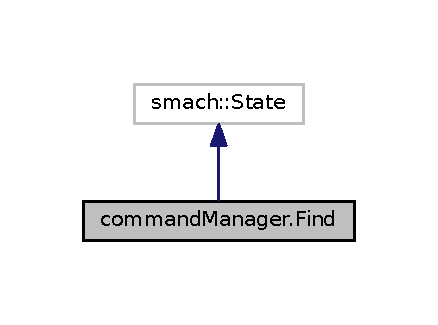
\includegraphics[width=210pt]{classcommandManager_1_1Find__inherit__graph}
\end{center}
\end{figure}


Collaboration diagram for command\+Manager.\+Find\+:\nopagebreak
\begin{figure}[H]
\begin{center}
\leavevmode
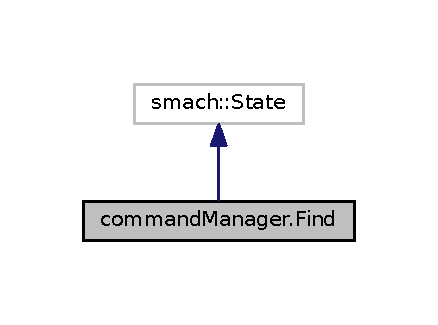
\includegraphics[width=210pt]{classcommandManager_1_1Find__coll__graph}
\end{center}
\end{figure}
\subsection*{Public Member Functions}
\begin{DoxyCompactItemize}
\item 
def \hyperlink{classcommandManager_1_1Find_ae547a564eeb683ea6d439cd8d0508779}{\+\_\+\+\_\+init\+\_\+\+\_\+} (self)
\item 
def \hyperlink{classcommandManager_1_1Find_aef4287ee7b2f43741e7dfd8d19b42878}{execute} (self, userdata)
\end{DoxyCompactItemize}
\subsection*{Public Attributes}
\begin{DoxyCompactItemize}
\item 
\hyperlink{classcommandManager_1_1Find_a75755e326232226bbd46786c7c889473}{counter}
\end{DoxyCompactItemize}
\subsection*{Static Public Attributes}
\begin{DoxyCompactItemize}
\item 
\hyperlink{classcommandManager_1_1Find_a9c7870d56b1d25a57af7840fb2967f99}{rate}
\end{DoxyCompactItemize}


\subsection{Detailed Description}
\begin{DoxyVerb}Class that defines the PLAY state. 
 It move the robot in X Y location and then asks to go back to the user.\end{DoxyVerb}
 

\subsection{Constructor \& Destructor Documentation}
\index{command\+Manager\+::\+Find@{command\+Manager\+::\+Find}!\+\_\+\+\_\+init\+\_\+\+\_\+@{\+\_\+\+\_\+init\+\_\+\+\_\+}}
\index{\+\_\+\+\_\+init\+\_\+\+\_\+@{\+\_\+\+\_\+init\+\_\+\+\_\+}!command\+Manager\+::\+Find@{command\+Manager\+::\+Find}}
\subsubsection[{\texorpdfstring{\+\_\+\+\_\+init\+\_\+\+\_\+(self)}{__init__(self)}}]{\setlength{\rightskip}{0pt plus 5cm}def command\+Manager.\+Find.\+\_\+\+\_\+init\+\_\+\+\_\+ (
\begin{DoxyParamCaption}
\item[{}]{self}
\end{DoxyParamCaption}
)}\hypertarget{classcommandManager_1_1Find_ae547a564eeb683ea6d439cd8d0508779}{}\label{classcommandManager_1_1Find_ae547a564eeb683ea6d439cd8d0508779}


\subsection{Member Function Documentation}
\index{command\+Manager\+::\+Find@{command\+Manager\+::\+Find}!execute@{execute}}
\index{execute@{execute}!command\+Manager\+::\+Find@{command\+Manager\+::\+Find}}
\subsubsection[{\texorpdfstring{execute(self, userdata)}{execute(self, userdata)}}]{\setlength{\rightskip}{0pt plus 5cm}def command\+Manager.\+Find.\+execute (
\begin{DoxyParamCaption}
\item[{}]{self, }
\item[{}]{userdata}
\end{DoxyParamCaption}
)}\hypertarget{classcommandManager_1_1Find_aef4287ee7b2f43741e7dfd8d19b42878}{}\label{classcommandManager_1_1Find_aef4287ee7b2f43741e7dfd8d19b42878}


\subsection{Member Data Documentation}
\index{command\+Manager\+::\+Find@{command\+Manager\+::\+Find}!counter@{counter}}
\index{counter@{counter}!command\+Manager\+::\+Find@{command\+Manager\+::\+Find}}
\subsubsection[{\texorpdfstring{counter}{counter}}]{\setlength{\rightskip}{0pt plus 5cm}command\+Manager.\+Find.\+counter}\hypertarget{classcommandManager_1_1Find_a75755e326232226bbd46786c7c889473}{}\label{classcommandManager_1_1Find_a75755e326232226bbd46786c7c889473}
\index{command\+Manager\+::\+Find@{command\+Manager\+::\+Find}!rate@{rate}}
\index{rate@{rate}!command\+Manager\+::\+Find@{command\+Manager\+::\+Find}}
\subsubsection[{\texorpdfstring{rate}{rate}}]{\setlength{\rightskip}{0pt plus 5cm}command\+Manager.\+Find.\+rate\hspace{0.3cm}{\ttfamily [static]}}\hypertarget{classcommandManager_1_1Find_a9c7870d56b1d25a57af7840fb2967f99}{}\label{classcommandManager_1_1Find_a9c7870d56b1d25a57af7840fb2967f99}


The documentation for this class was generated from the following file\+:\begin{DoxyCompactItemize}
\item 
/home/francescotesta/experimental\+\_\+ws/src/final\+\_\+assignment/scripts/\hyperlink{commandManager_8py}{command\+Manager.\+py}\end{DoxyCompactItemize}

\hypertarget{classnoSleep_1_1Find}{}\section{no\+Sleep.\+Find Class Reference}
\label{classnoSleep_1_1Find}\index{no\+Sleep.\+Find@{no\+Sleep.\+Find}}


Inheritance diagram for no\+Sleep.\+Find\+:\nopagebreak
\begin{figure}[H]
\begin{center}
\leavevmode
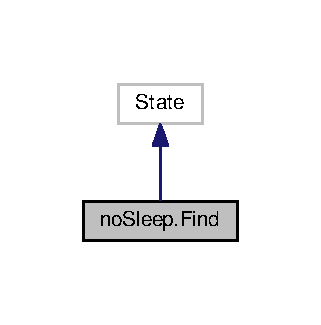
\includegraphics[width=154pt]{classnoSleep_1_1Find__inherit__graph}
\end{center}
\end{figure}


Collaboration diagram for no\+Sleep.\+Find\+:\nopagebreak
\begin{figure}[H]
\begin{center}
\leavevmode
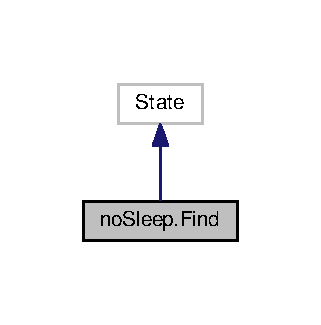
\includegraphics[width=154pt]{classnoSleep_1_1Find__coll__graph}
\end{center}
\end{figure}
\subsection*{Public Member Functions}
\begin{DoxyCompactItemize}
\item 
def \hyperlink{classnoSleep_1_1Find_aff34d2da153e2a1aff424ec9a02dcdb2}{\+\_\+\+\_\+init\+\_\+\+\_\+} (self)
\item 
def \hyperlink{classnoSleep_1_1Find_a3a023c41893fa105656edec93c0891cf}{execute} (self, userdata)
\end{DoxyCompactItemize}
\subsection*{Static Public Attributes}
\begin{DoxyCompactItemize}
\item 
\hyperlink{classnoSleep_1_1Find_a29d9bba04c1821d063ab293ef4512b02}{rate}
\item 
\hyperlink{classnoSleep_1_1Find_a3b10497b340f42598a97d7dc4c3823a6}{pos} = rooms.\+explore()
\end{DoxyCompactItemize}


\subsection{Detailed Description}
\begin{DoxyVerb}Class that defines the FIND state. 
 It move the robot using the explore function in order to find the esired room or a new one.\end{DoxyVerb}
 

\subsection{Constructor \& Destructor Documentation}
\index{no\+Sleep\+::\+Find@{no\+Sleep\+::\+Find}!\+\_\+\+\_\+init\+\_\+\+\_\+@{\+\_\+\+\_\+init\+\_\+\+\_\+}}
\index{\+\_\+\+\_\+init\+\_\+\+\_\+@{\+\_\+\+\_\+init\+\_\+\+\_\+}!no\+Sleep\+::\+Find@{no\+Sleep\+::\+Find}}
\subsubsection[{\texorpdfstring{\+\_\+\+\_\+init\+\_\+\+\_\+(self)}{__init__(self)}}]{\setlength{\rightskip}{0pt plus 5cm}def no\+Sleep.\+Find.\+\_\+\+\_\+init\+\_\+\+\_\+ (
\begin{DoxyParamCaption}
\item[{}]{self}
\end{DoxyParamCaption}
)}\hypertarget{classnoSleep_1_1Find_aff34d2da153e2a1aff424ec9a02dcdb2}{}\label{classnoSleep_1_1Find_aff34d2da153e2a1aff424ec9a02dcdb2}


\subsection{Member Function Documentation}
\index{no\+Sleep\+::\+Find@{no\+Sleep\+::\+Find}!execute@{execute}}
\index{execute@{execute}!no\+Sleep\+::\+Find@{no\+Sleep\+::\+Find}}
\subsubsection[{\texorpdfstring{execute(self, userdata)}{execute(self, userdata)}}]{\setlength{\rightskip}{0pt plus 5cm}def no\+Sleep.\+Find.\+execute (
\begin{DoxyParamCaption}
\item[{}]{self, }
\item[{}]{userdata}
\end{DoxyParamCaption}
)}\hypertarget{classnoSleep_1_1Find_a3a023c41893fa105656edec93c0891cf}{}\label{classnoSleep_1_1Find_a3a023c41893fa105656edec93c0891cf}


\subsection{Member Data Documentation}
\index{no\+Sleep\+::\+Find@{no\+Sleep\+::\+Find}!pos@{pos}}
\index{pos@{pos}!no\+Sleep\+::\+Find@{no\+Sleep\+::\+Find}}
\subsubsection[{\texorpdfstring{pos}{pos}}]{\setlength{\rightskip}{0pt plus 5cm}no\+Sleep.\+Find.\+pos = rooms.\+explore()\hspace{0.3cm}{\ttfamily [static]}}\hypertarget{classnoSleep_1_1Find_a3b10497b340f42598a97d7dc4c3823a6}{}\label{classnoSleep_1_1Find_a3b10497b340f42598a97d7dc4c3823a6}
\index{no\+Sleep\+::\+Find@{no\+Sleep\+::\+Find}!rate@{rate}}
\index{rate@{rate}!no\+Sleep\+::\+Find@{no\+Sleep\+::\+Find}}
\subsubsection[{\texorpdfstring{rate}{rate}}]{\setlength{\rightskip}{0pt plus 5cm}no\+Sleep.\+Find.\+rate\hspace{0.3cm}{\ttfamily [static]}}\hypertarget{classnoSleep_1_1Find_a29d9bba04c1821d063ab293ef4512b02}{}\label{classnoSleep_1_1Find_a29d9bba04c1821d063ab293ef4512b02}


The documentation for this class was generated from the following file\+:\begin{DoxyCompactItemize}
\item 
/home/francescotesta/experimental\+\_\+ws/src/final\+\_\+assignment/scripts/\hyperlink{noSleep_8py}{no\+Sleep.\+py}\end{DoxyCompactItemize}

\hypertarget{classcommandManager_1_1Normal}{}\section{command\+Manager.\+Normal Class Reference}
\label{classcommandManager_1_1Normal}\index{command\+Manager.\+Normal@{command\+Manager.\+Normal}}


Inheritance diagram for command\+Manager.\+Normal\+:\nopagebreak
\begin{figure}[H]
\begin{center}
\leavevmode
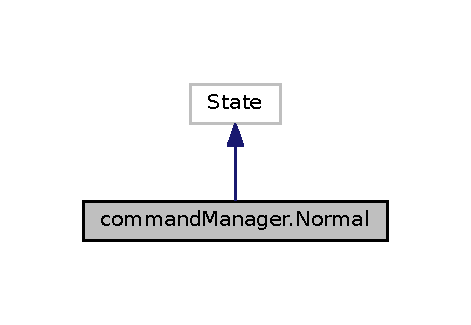
\includegraphics[width=226pt]{classcommandManager_1_1Normal__inherit__graph}
\end{center}
\end{figure}


Collaboration diagram for command\+Manager.\+Normal\+:\nopagebreak
\begin{figure}[H]
\begin{center}
\leavevmode
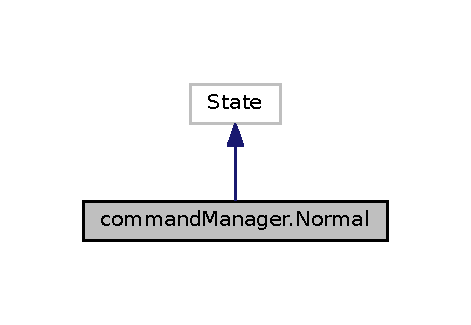
\includegraphics[width=226pt]{classcommandManager_1_1Normal__coll__graph}
\end{center}
\end{figure}
\subsection*{Public Member Functions}
\begin{DoxyCompactItemize}
\item 
def \hyperlink{classcommandManager_1_1Normal_abda69ab53b7d84c2c0c577dcf26f3823}{\+\_\+\+\_\+init\+\_\+\+\_\+} (self)
\item 
def \hyperlink{classcommandManager_1_1Normal_ae95451bab37e817557988c7190bb33bd}{execute} (self, userdata)
\end{DoxyCompactItemize}
\subsection*{Public Attributes}
\begin{DoxyCompactItemize}
\item 
\hyperlink{classcommandManager_1_1Normal_a32e84cf5ac08ffeb9cb1a21d4b484a32}{rate}
\end{DoxyCompactItemize}
\subsection*{Static Public Attributes}
\begin{DoxyCompactItemize}
\item 
\hyperlink{classcommandManager_1_1Normal_a5ebc9e1cc3847edb576acedd01487023}{counter}
\begin{DoxyCompactList}\small\item\em Counter variable to check the number of iteration of the N\+O\+R\+M\+AL state in order to move to S\+L\+E\+EP state after a certain number. \end{DoxyCompactList}\item 
\hyperlink{classcommandManager_1_1Normal_a160432e70539a4ac4dd4a5bf733824a3}{pos} = rooms.\+generate\+\_\+rand\+\_\+pos()
\end{DoxyCompactItemize}


\subsection{Detailed Description}
\begin{DoxyVerb}This class defines the NORMAL state of the FSM. In particular It sends random position to the navigation_action server
and it checks whether a ball is detected in order to move to PLAY state.
Otherwise after some iterations it goes in SLEEP mode \end{DoxyVerb}
 

\subsection{Constructor \& Destructor Documentation}
\index{command\+Manager\+::\+Normal@{command\+Manager\+::\+Normal}!\+\_\+\+\_\+init\+\_\+\+\_\+@{\+\_\+\+\_\+init\+\_\+\+\_\+}}
\index{\+\_\+\+\_\+init\+\_\+\+\_\+@{\+\_\+\+\_\+init\+\_\+\+\_\+}!command\+Manager\+::\+Normal@{command\+Manager\+::\+Normal}}
\subsubsection[{\texorpdfstring{\+\_\+\+\_\+init\+\_\+\+\_\+(self)}{__init__(self)}}]{\setlength{\rightskip}{0pt plus 5cm}def command\+Manager.\+Normal.\+\_\+\+\_\+init\+\_\+\+\_\+ (
\begin{DoxyParamCaption}
\item[{}]{self}
\end{DoxyParamCaption}
)}\hypertarget{classcommandManager_1_1Normal_abda69ab53b7d84c2c0c577dcf26f3823}{}\label{classcommandManager_1_1Normal_abda69ab53b7d84c2c0c577dcf26f3823}


\subsection{Member Function Documentation}
\index{command\+Manager\+::\+Normal@{command\+Manager\+::\+Normal}!execute@{execute}}
\index{execute@{execute}!command\+Manager\+::\+Normal@{command\+Manager\+::\+Normal}}
\subsubsection[{\texorpdfstring{execute(self, userdata)}{execute(self, userdata)}}]{\setlength{\rightskip}{0pt plus 5cm}def command\+Manager.\+Normal.\+execute (
\begin{DoxyParamCaption}
\item[{}]{self, }
\item[{}]{userdata}
\end{DoxyParamCaption}
)}\hypertarget{classcommandManager_1_1Normal_ae95451bab37e817557988c7190bb33bd}{}\label{classcommandManager_1_1Normal_ae95451bab37e817557988c7190bb33bd}


\subsection{Member Data Documentation}
\index{command\+Manager\+::\+Normal@{command\+Manager\+::\+Normal}!counter@{counter}}
\index{counter@{counter}!command\+Manager\+::\+Normal@{command\+Manager\+::\+Normal}}
\subsubsection[{\texorpdfstring{counter}{counter}}]{\setlength{\rightskip}{0pt plus 5cm}command\+Manager.\+Normal.\+counter\hspace{0.3cm}{\ttfamily [static]}}\hypertarget{classcommandManager_1_1Normal_a5ebc9e1cc3847edb576acedd01487023}{}\label{classcommandManager_1_1Normal_a5ebc9e1cc3847edb576acedd01487023}


Counter variable to check the number of iteration of the N\+O\+R\+M\+AL state in order to move to S\+L\+E\+EP state after a certain number. 

\index{command\+Manager\+::\+Normal@{command\+Manager\+::\+Normal}!pos@{pos}}
\index{pos@{pos}!command\+Manager\+::\+Normal@{command\+Manager\+::\+Normal}}
\subsubsection[{\texorpdfstring{pos}{pos}}]{\setlength{\rightskip}{0pt plus 5cm}command\+Manager.\+Normal.\+pos = rooms.\+generate\+\_\+rand\+\_\+pos()\hspace{0.3cm}{\ttfamily [static]}}\hypertarget{classcommandManager_1_1Normal_a160432e70539a4ac4dd4a5bf733824a3}{}\label{classcommandManager_1_1Normal_a160432e70539a4ac4dd4a5bf733824a3}
\index{command\+Manager\+::\+Normal@{command\+Manager\+::\+Normal}!rate@{rate}}
\index{rate@{rate}!command\+Manager\+::\+Normal@{command\+Manager\+::\+Normal}}
\subsubsection[{\texorpdfstring{rate}{rate}}]{\setlength{\rightskip}{0pt plus 5cm}command\+Manager.\+Normal.\+rate}\hypertarget{classcommandManager_1_1Normal_a32e84cf5ac08ffeb9cb1a21d4b484a32}{}\label{classcommandManager_1_1Normal_a32e84cf5ac08ffeb9cb1a21d4b484a32}


The documentation for this class was generated from the following file\+:\begin{DoxyCompactItemize}
\item 
/home/francescotesta/experimental\+\_\+ws/src/final\+\_\+assignment/scripts/\hyperlink{commandManager_8py}{command\+Manager.\+py}\end{DoxyCompactItemize}

\hypertarget{classnoSleep_1_1Normal}{}\section{no\+Sleep.\+Normal Class Reference}
\label{classnoSleep_1_1Normal}\index{no\+Sleep.\+Normal@{no\+Sleep.\+Normal}}


Inheritance diagram for no\+Sleep.\+Normal\+:\nopagebreak
\begin{figure}[H]
\begin{center}
\leavevmode
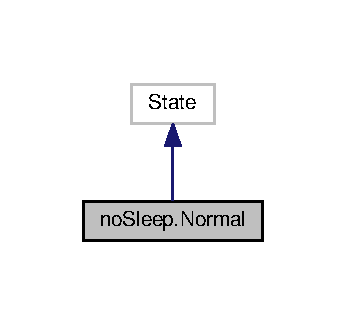
\includegraphics[width=166pt]{classnoSleep_1_1Normal__inherit__graph}
\end{center}
\end{figure}


Collaboration diagram for no\+Sleep.\+Normal\+:\nopagebreak
\begin{figure}[H]
\begin{center}
\leavevmode
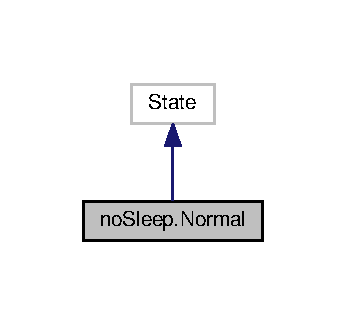
\includegraphics[width=166pt]{classnoSleep_1_1Normal__coll__graph}
\end{center}
\end{figure}
\subsection*{Public Member Functions}
\begin{DoxyCompactItemize}
\item 
def \hyperlink{classnoSleep_1_1Normal_a408dace152fbaea3a755a27ded06b1a5}{\+\_\+\+\_\+init\+\_\+\+\_\+} (self)
\item 
def \hyperlink{classnoSleep_1_1Normal_ad4ca86ae46f2a71c2e8fc58efeb6e152}{execute} (self, userdata)
\end{DoxyCompactItemize}
\subsection*{Static Public Attributes}
\begin{DoxyCompactItemize}
\item 
\hyperlink{classnoSleep_1_1Normal_ac888ccee4346d4596fc6d96d1659afa1}{rate}
\item 
\hyperlink{classnoSleep_1_1Normal_aa10f1e841df545b9ae37ccab18807937}{counter}
\begin{DoxyCompactList}\small\item\em Counter variable to check the number of iteration of the N\+O\+R\+M\+AL state in order to move to S\+L\+E\+EP state after a certain number. \end{DoxyCompactList}\item 
\hyperlink{classnoSleep_1_1Normal_acd333157173f8328e1e0f62d2e57e157}{pos} = rooms.\+generate\+\_\+rand\+\_\+pos()
\end{DoxyCompactItemize}


\subsection{Detailed Description}
\begin{DoxyVerb}This class defines the NORMAL state of the FSM. In particular It sends random position to the move_base action server.
It checks whether a ball is detected in order to switch in the TRACK state and check if the user wants to switch in the PLAY state as well.
Otherwise after some iterations it goes in SLEEP mode 
\end{DoxyVerb}
 

\subsection{Constructor \& Destructor Documentation}
\index{no\+Sleep\+::\+Normal@{no\+Sleep\+::\+Normal}!\+\_\+\+\_\+init\+\_\+\+\_\+@{\+\_\+\+\_\+init\+\_\+\+\_\+}}
\index{\+\_\+\+\_\+init\+\_\+\+\_\+@{\+\_\+\+\_\+init\+\_\+\+\_\+}!no\+Sleep\+::\+Normal@{no\+Sleep\+::\+Normal}}
\subsubsection[{\texorpdfstring{\+\_\+\+\_\+init\+\_\+\+\_\+(self)}{__init__(self)}}]{\setlength{\rightskip}{0pt plus 5cm}def no\+Sleep.\+Normal.\+\_\+\+\_\+init\+\_\+\+\_\+ (
\begin{DoxyParamCaption}
\item[{}]{self}
\end{DoxyParamCaption}
)}\hypertarget{classnoSleep_1_1Normal_a408dace152fbaea3a755a27ded06b1a5}{}\label{classnoSleep_1_1Normal_a408dace152fbaea3a755a27ded06b1a5}


\subsection{Member Function Documentation}
\index{no\+Sleep\+::\+Normal@{no\+Sleep\+::\+Normal}!execute@{execute}}
\index{execute@{execute}!no\+Sleep\+::\+Normal@{no\+Sleep\+::\+Normal}}
\subsubsection[{\texorpdfstring{execute(self, userdata)}{execute(self, userdata)}}]{\setlength{\rightskip}{0pt plus 5cm}def no\+Sleep.\+Normal.\+execute (
\begin{DoxyParamCaption}
\item[{}]{self, }
\item[{}]{userdata}
\end{DoxyParamCaption}
)}\hypertarget{classnoSleep_1_1Normal_ad4ca86ae46f2a71c2e8fc58efeb6e152}{}\label{classnoSleep_1_1Normal_ad4ca86ae46f2a71c2e8fc58efeb6e152}


\subsection{Member Data Documentation}
\index{no\+Sleep\+::\+Normal@{no\+Sleep\+::\+Normal}!counter@{counter}}
\index{counter@{counter}!no\+Sleep\+::\+Normal@{no\+Sleep\+::\+Normal}}
\subsubsection[{\texorpdfstring{counter}{counter}}]{\setlength{\rightskip}{0pt plus 5cm}no\+Sleep.\+Normal.\+counter\hspace{0.3cm}{\ttfamily [static]}}\hypertarget{classnoSleep_1_1Normal_aa10f1e841df545b9ae37ccab18807937}{}\label{classnoSleep_1_1Normal_aa10f1e841df545b9ae37ccab18807937}


Counter variable to check the number of iteration of the N\+O\+R\+M\+AL state in order to move to S\+L\+E\+EP state after a certain number. 

\index{no\+Sleep\+::\+Normal@{no\+Sleep\+::\+Normal}!pos@{pos}}
\index{pos@{pos}!no\+Sleep\+::\+Normal@{no\+Sleep\+::\+Normal}}
\subsubsection[{\texorpdfstring{pos}{pos}}]{\setlength{\rightskip}{0pt plus 5cm}no\+Sleep.\+Normal.\+pos = rooms.\+generate\+\_\+rand\+\_\+pos()\hspace{0.3cm}{\ttfamily [static]}}\hypertarget{classnoSleep_1_1Normal_acd333157173f8328e1e0f62d2e57e157}{}\label{classnoSleep_1_1Normal_acd333157173f8328e1e0f62d2e57e157}
\begin{DoxyVerb}Method inherited from the smach.State class \end{DoxyVerb}
 \index{no\+Sleep\+::\+Normal@{no\+Sleep\+::\+Normal}!rate@{rate}}
\index{rate@{rate}!no\+Sleep\+::\+Normal@{no\+Sleep\+::\+Normal}}
\subsubsection[{\texorpdfstring{rate}{rate}}]{\setlength{\rightskip}{0pt plus 5cm}no\+Sleep.\+Normal.\+rate\hspace{0.3cm}{\ttfamily [static]}}\hypertarget{classnoSleep_1_1Normal_ac888ccee4346d4596fc6d96d1659afa1}{}\label{classnoSleep_1_1Normal_ac888ccee4346d4596fc6d96d1659afa1}


The documentation for this class was generated from the following file\+:\begin{DoxyCompactItemize}
\item 
/home/francescotesta/experimental\+\_\+ws/src/final\+\_\+assignment/scripts/\hyperlink{noSleep_8py}{no\+Sleep.\+py}\end{DoxyCompactItemize}

\hypertarget{classnoSleep_1_1Play}{}\section{no\+Sleep.\+Play Class Reference}
\label{classnoSleep_1_1Play}\index{no\+Sleep.\+Play@{no\+Sleep.\+Play}}


Inheritance diagram for no\+Sleep.\+Play\+:\nopagebreak
\begin{figure}[H]
\begin{center}
\leavevmode
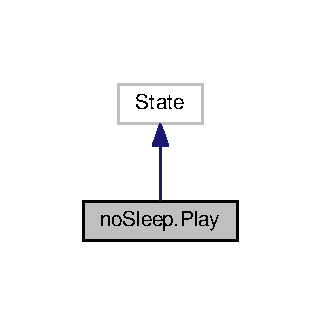
\includegraphics[width=154pt]{classnoSleep_1_1Play__inherit__graph}
\end{center}
\end{figure}


Collaboration diagram for no\+Sleep.\+Play\+:\nopagebreak
\begin{figure}[H]
\begin{center}
\leavevmode
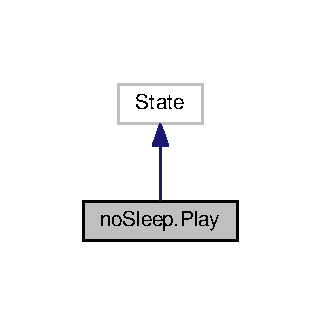
\includegraphics[width=154pt]{classnoSleep_1_1Play__coll__graph}
\end{center}
\end{figure}
\subsection*{Public Member Functions}
\begin{DoxyCompactItemize}
\item 
def \hyperlink{classnoSleep_1_1Play_a587a6f6981b7b8b741ffba66fbad8ded}{\+\_\+\+\_\+init\+\_\+\+\_\+} (self)
\item 
def \hyperlink{classnoSleep_1_1Play_ab0ab4ba67c0feb27958d4f6655f9e104}{execute} (self, userdata)
\end{DoxyCompactItemize}
\subsection*{Public Attributes}
\begin{DoxyCompactItemize}
\item 
\hyperlink{classnoSleep_1_1Play_af1b7d964b638181e21fb682f418e6b6e}{rate}
\end{DoxyCompactItemize}
\subsection*{Static Public Attributes}
\begin{DoxyCompactItemize}
\item 
\hyperlink{classnoSleep_1_1Play_a79d30952a61e9c2b272bbbe28efc81f2}{counter}
\begin{DoxyCompactList}\small\item\em Variable to count the time pass. \end{DoxyCompactList}\item 
\hyperlink{classnoSleep_1_1Play_adeeb3f6ce6c5df5baa3bf6399dfbe2bb}{position} = rooms.\+get\+\_\+room\+\_\+position(\char`\"{}Home\char`\"{})
\end{DoxyCompactItemize}


\subsection{Detailed Description}
\begin{DoxyVerb}Class that defines the PLAY state. 
 It move the robot in X Y location and then asks to go back to the user.\end{DoxyVerb}
 

\subsection{Constructor \& Destructor Documentation}
\index{no\+Sleep\+::\+Play@{no\+Sleep\+::\+Play}!\+\_\+\+\_\+init\+\_\+\+\_\+@{\+\_\+\+\_\+init\+\_\+\+\_\+}}
\index{\+\_\+\+\_\+init\+\_\+\+\_\+@{\+\_\+\+\_\+init\+\_\+\+\_\+}!no\+Sleep\+::\+Play@{no\+Sleep\+::\+Play}}
\subsubsection[{\texorpdfstring{\+\_\+\+\_\+init\+\_\+\+\_\+(self)}{__init__(self)}}]{\setlength{\rightskip}{0pt plus 5cm}def no\+Sleep.\+Play.\+\_\+\+\_\+init\+\_\+\+\_\+ (
\begin{DoxyParamCaption}
\item[{}]{self}
\end{DoxyParamCaption}
)}\hypertarget{classnoSleep_1_1Play_a587a6f6981b7b8b741ffba66fbad8ded}{}\label{classnoSleep_1_1Play_a587a6f6981b7b8b741ffba66fbad8ded}
\begin{DoxyVerb}Class that defines the PLAY state. 
 It move the robot in X Y location and then asks to go back to the user.\end{DoxyVerb}
 

\subsection{Member Function Documentation}
\index{no\+Sleep\+::\+Play@{no\+Sleep\+::\+Play}!execute@{execute}}
\index{execute@{execute}!no\+Sleep\+::\+Play@{no\+Sleep\+::\+Play}}
\subsubsection[{\texorpdfstring{execute(self, userdata)}{execute(self, userdata)}}]{\setlength{\rightskip}{0pt plus 5cm}def no\+Sleep.\+Play.\+execute (
\begin{DoxyParamCaption}
\item[{}]{self, }
\item[{}]{userdata}
\end{DoxyParamCaption}
)}\hypertarget{classnoSleep_1_1Play_ab0ab4ba67c0feb27958d4f6655f9e104}{}\label{classnoSleep_1_1Play_ab0ab4ba67c0feb27958d4f6655f9e104}


\subsection{Member Data Documentation}
\index{no\+Sleep\+::\+Play@{no\+Sleep\+::\+Play}!counter@{counter}}
\index{counter@{counter}!no\+Sleep\+::\+Play@{no\+Sleep\+::\+Play}}
\subsubsection[{\texorpdfstring{counter}{counter}}]{\setlength{\rightskip}{0pt plus 5cm}no\+Sleep.\+Play.\+counter\hspace{0.3cm}{\ttfamily [static]}}\hypertarget{classnoSleep_1_1Play_a79d30952a61e9c2b272bbbe28efc81f2}{}\label{classnoSleep_1_1Play_a79d30952a61e9c2b272bbbe28efc81f2}


Variable to count the time pass. 

\index{no\+Sleep\+::\+Play@{no\+Sleep\+::\+Play}!position@{position}}
\index{position@{position}!no\+Sleep\+::\+Play@{no\+Sleep\+::\+Play}}
\subsubsection[{\texorpdfstring{position}{position}}]{\setlength{\rightskip}{0pt plus 5cm}no\+Sleep.\+Play.\+position = rooms.\+get\+\_\+room\+\_\+position(\char`\"{}Home\char`\"{})\hspace{0.3cm}{\ttfamily [static]}}\hypertarget{classnoSleep_1_1Play_adeeb3f6ce6c5df5baa3bf6399dfbe2bb}{}\label{classnoSleep_1_1Play_adeeb3f6ce6c5df5baa3bf6399dfbe2bb}
\index{no\+Sleep\+::\+Play@{no\+Sleep\+::\+Play}!rate@{rate}}
\index{rate@{rate}!no\+Sleep\+::\+Play@{no\+Sleep\+::\+Play}}
\subsubsection[{\texorpdfstring{rate}{rate}}]{\setlength{\rightskip}{0pt plus 5cm}no\+Sleep.\+Play.\+rate}\hypertarget{classnoSleep_1_1Play_af1b7d964b638181e21fb682f418e6b6e}{}\label{classnoSleep_1_1Play_af1b7d964b638181e21fb682f418e6b6e}


The documentation for this class was generated from the following file\+:\begin{DoxyCompactItemize}
\item 
/home/francescotesta/experimental\+\_\+ws/src/final\+\_\+assignment/scripts/\hyperlink{noSleep_8py}{no\+Sleep.\+py}\end{DoxyCompactItemize}

\hypertarget{classcommandManager_1_1Play}{}\section{command\+Manager.\+Play Class Reference}
\label{classcommandManager_1_1Play}\index{command\+Manager.\+Play@{command\+Manager.\+Play}}


Inheritance diagram for command\+Manager.\+Play\+:\nopagebreak
\begin{figure}[H]
\begin{center}
\leavevmode
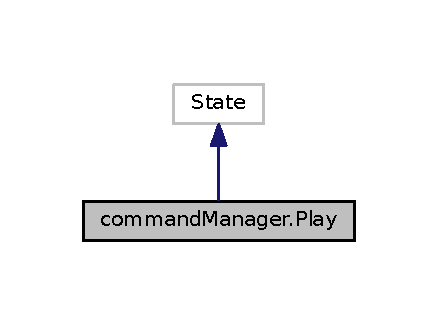
\includegraphics[width=210pt]{classcommandManager_1_1Play__inherit__graph}
\end{center}
\end{figure}


Collaboration diagram for command\+Manager.\+Play\+:\nopagebreak
\begin{figure}[H]
\begin{center}
\leavevmode
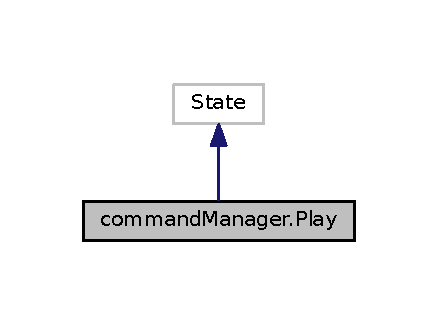
\includegraphics[width=210pt]{classcommandManager_1_1Play__coll__graph}
\end{center}
\end{figure}
\subsection*{Public Member Functions}
\begin{DoxyCompactItemize}
\item 
def \hyperlink{classcommandManager_1_1Play_a4bc5c3700d80432b4dd09b163f210540}{\+\_\+\+\_\+init\+\_\+\+\_\+} (self)
\item 
def \hyperlink{classcommandManager_1_1Play_a2ec6a287ce47f3f6c08c76cc452cf4d3}{execute} (self, userdata)
\end{DoxyCompactItemize}
\subsection*{Public Attributes}
\begin{DoxyCompactItemize}
\item 
\hyperlink{classcommandManager_1_1Play_a34aba8df5dfec3560f194934b7e377ad}{rate}
\end{DoxyCompactItemize}
\subsection*{Static Public Attributes}
\begin{DoxyCompactItemize}
\item 
\hyperlink{classcommandManager_1_1Play_a0999085c98a27adf5b79df2691a7e222}{counter}
\begin{DoxyCompactList}\small\item\em Variable to count the time pass. \end{DoxyCompactList}\item 
\hyperlink{classcommandManager_1_1Play_a0cd6441e9cc0ec9ec7acb974b5b1354e}{position} = rooms.\+get\+\_\+room\+\_\+position(\char`\"{}Home\char`\"{})
\end{DoxyCompactItemize}


\subsection{Detailed Description}
\begin{DoxyVerb}Class that defines the PLAY state. 
 It move the robot in X Y location and then asks to go back to the user.\end{DoxyVerb}
 

\subsection{Constructor \& Destructor Documentation}
\index{command\+Manager\+::\+Play@{command\+Manager\+::\+Play}!\+\_\+\+\_\+init\+\_\+\+\_\+@{\+\_\+\+\_\+init\+\_\+\+\_\+}}
\index{\+\_\+\+\_\+init\+\_\+\+\_\+@{\+\_\+\+\_\+init\+\_\+\+\_\+}!command\+Manager\+::\+Play@{command\+Manager\+::\+Play}}
\subsubsection[{\texorpdfstring{\+\_\+\+\_\+init\+\_\+\+\_\+(self)}{__init__(self)}}]{\setlength{\rightskip}{0pt plus 5cm}def command\+Manager.\+Play.\+\_\+\+\_\+init\+\_\+\+\_\+ (
\begin{DoxyParamCaption}
\item[{}]{self}
\end{DoxyParamCaption}
)}\hypertarget{classcommandManager_1_1Play_a4bc5c3700d80432b4dd09b163f210540}{}\label{classcommandManager_1_1Play_a4bc5c3700d80432b4dd09b163f210540}
\begin{DoxyVerb}Class that defines the PLAY state. 
 It move the robot in X Y location and then asks to go back to the user.\end{DoxyVerb}
 

\subsection{Member Function Documentation}
\index{command\+Manager\+::\+Play@{command\+Manager\+::\+Play}!execute@{execute}}
\index{execute@{execute}!command\+Manager\+::\+Play@{command\+Manager\+::\+Play}}
\subsubsection[{\texorpdfstring{execute(self, userdata)}{execute(self, userdata)}}]{\setlength{\rightskip}{0pt plus 5cm}def command\+Manager.\+Play.\+execute (
\begin{DoxyParamCaption}
\item[{}]{self, }
\item[{}]{userdata}
\end{DoxyParamCaption}
)}\hypertarget{classcommandManager_1_1Play_a2ec6a287ce47f3f6c08c76cc452cf4d3}{}\label{classcommandManager_1_1Play_a2ec6a287ce47f3f6c08c76cc452cf4d3}


\subsection{Member Data Documentation}
\index{command\+Manager\+::\+Play@{command\+Manager\+::\+Play}!counter@{counter}}
\index{counter@{counter}!command\+Manager\+::\+Play@{command\+Manager\+::\+Play}}
\subsubsection[{\texorpdfstring{counter}{counter}}]{\setlength{\rightskip}{0pt plus 5cm}command\+Manager.\+Play.\+counter\hspace{0.3cm}{\ttfamily [static]}}\hypertarget{classcommandManager_1_1Play_a0999085c98a27adf5b79df2691a7e222}{}\label{classcommandManager_1_1Play_a0999085c98a27adf5b79df2691a7e222}


Variable to count the time pass. 

\index{command\+Manager\+::\+Play@{command\+Manager\+::\+Play}!position@{position}}
\index{position@{position}!command\+Manager\+::\+Play@{command\+Manager\+::\+Play}}
\subsubsection[{\texorpdfstring{position}{position}}]{\setlength{\rightskip}{0pt plus 5cm}command\+Manager.\+Play.\+position = rooms.\+get\+\_\+room\+\_\+position(\char`\"{}Home\char`\"{})\hspace{0.3cm}{\ttfamily [static]}}\hypertarget{classcommandManager_1_1Play_a0cd6441e9cc0ec9ec7acb974b5b1354e}{}\label{classcommandManager_1_1Play_a0cd6441e9cc0ec9ec7acb974b5b1354e}
\index{command\+Manager\+::\+Play@{command\+Manager\+::\+Play}!rate@{rate}}
\index{rate@{rate}!command\+Manager\+::\+Play@{command\+Manager\+::\+Play}}
\subsubsection[{\texorpdfstring{rate}{rate}}]{\setlength{\rightskip}{0pt plus 5cm}command\+Manager.\+Play.\+rate}\hypertarget{classcommandManager_1_1Play_a34aba8df5dfec3560f194934b7e377ad}{}\label{classcommandManager_1_1Play_a34aba8df5dfec3560f194934b7e377ad}


The documentation for this class was generated from the following file\+:\begin{DoxyCompactItemize}
\item 
/home/francescotesta/experimental\+\_\+ws/src/final\+\_\+assignment/scripts/\hyperlink{commandManager_8py}{command\+Manager.\+py}\end{DoxyCompactItemize}

\hypertarget{classroomDetector_1_1roomDetector}{}\section{room\+Detector.\+room\+Detector Class Reference}
\label{classroomDetector_1_1roomDetector}\index{room\+Detector.\+room\+Detector@{room\+Detector.\+room\+Detector}}


This class implements a subscriber to the camera topic of the robot and applies several open\+CV mask in order to recognise the color of the ball, then it send the detected color to the \hyperlink{namespacecommandManager}{command\+Manager} node.  


\subsection*{Public Member Functions}
\begin{DoxyCompactItemize}
\item 
def \hyperlink{classroomDetector_1_1roomDetector_a1038f6f11c424041c0d9584b6f9c6833}{\+\_\+\+\_\+init\+\_\+\+\_\+} (self)
\item 
def \hyperlink{classroomDetector_1_1roomDetector_a4c27707debecd7e07f55f0e66f460b37}{find\+\_\+color} (self, hsv\+\_\+min, hsv\+\_\+max, image\+\_\+np)
\begin{DoxyCompactList}\small\item\em Method returns True when a ball is detected. \end{DoxyCompactList}\item 
def \hyperlink{classroomDetector_1_1roomDetector_a6c045c0740ea0cee247c81d20a9d1c91}{find\+\_\+ball} (self, ros\+\_\+image)
\begin{DoxyCompactList}\small\item\em Callback method for the image camera subscriber, so it\textquotesingle{}s called everytime a new image is available. \end{DoxyCompactList}\item 
def \hyperlink{classroomDetector_1_1roomDetector_aa8a2aea1db8ce538d11ddb501fae2822}{start\+Detection} (self)
\begin{DoxyCompactList}\small\item\em Start the subscriber to the camera topic, thus the node starts to detect balls. \end{DoxyCompactList}\item 
def \hyperlink{classroomDetector_1_1roomDetector_a1b30655196cae01d824ddeab2bb7e0e3}{stop\+Detection} (self)
\begin{DoxyCompactList}\small\item\em Intterrupt the subsciption to the camera topic. \end{DoxyCompactList}\end{DoxyCompactItemize}
\subsection*{Static Public Attributes}
\begin{DoxyCompactItemize}
\item 
\hyperlink{classroomDetector_1_1roomDetector_ac3ba7d2b6d48205de38cd18b333237d6}{anonymous}
\item 
\hyperlink{classroomDetector_1_1roomDetector_a1e899d16548ade375ed0b0dc6e1d9d98}{prev\+Color}
\begin{DoxyCompactList}\small\item\em Contains the previously detected color in order to avoid notifying the same room several times, when the robot starts to track it. \end{DoxyCompactList}\item 
\hyperlink{classroomDetector_1_1roomDetector_a35a2705eee8284eaad169dd0830fc6de}{new\+Room\+Pub}
\begin{DoxyCompactList}\small\item\em Subsriber to get the compressed images from the robot camera. \end{DoxyCompactList}\item 
\hyperlink{classroomDetector_1_1roomDetector_a14b6749ddaf264a41497904c0513ed9b}{String}
\item 
\hyperlink{classroomDetector_1_1roomDetector_a86aaaea08936260cb6e591c10b0dfeae}{queue\+\_\+size}
\item 
\hyperlink{classroomDetector_1_1roomDetector_ad3dbc1e4c7a827af098c86101198a1f4}{rate}
\item 
\hyperlink{classroomDetector_1_1roomDetector_a2a904c657007f56412c9e495cc254cad}{ball\+Detected}
\item 
\hyperlink{classroomDetector_1_1roomDetector_a0a32f7c136b2b46325c0e36275c6fb57}{camera\+\_\+sub}
\item 
\hyperlink{classroomDetector_1_1roomDetector_a86847f178ca59553c205557f2de199d8}{find\+\_\+ball}
\end{DoxyCompactItemize}


\subsection{Detailed Description}
This class implements a subscriber to the camera topic of the robot and applies several open\+CV mask in order to recognise the color of the ball, then it send the detected color to the \hyperlink{namespacecommandManager}{command\+Manager} node. 



\subsection{Constructor \& Destructor Documentation}
\index{room\+Detector\+::room\+Detector@{room\+Detector\+::room\+Detector}!\+\_\+\+\_\+init\+\_\+\+\_\+@{\+\_\+\+\_\+init\+\_\+\+\_\+}}
\index{\+\_\+\+\_\+init\+\_\+\+\_\+@{\+\_\+\+\_\+init\+\_\+\+\_\+}!room\+Detector\+::room\+Detector@{room\+Detector\+::room\+Detector}}
\subsubsection[{\texorpdfstring{\+\_\+\+\_\+init\+\_\+\+\_\+(self)}{__init__(self)}}]{\setlength{\rightskip}{0pt plus 5cm}def room\+Detector.\+room\+Detector.\+\_\+\+\_\+init\+\_\+\+\_\+ (
\begin{DoxyParamCaption}
\item[{}]{self}
\end{DoxyParamCaption}
)}\hypertarget{classroomDetector_1_1roomDetector_a1038f6f11c424041c0d9584b6f9c6833}{}\label{classroomDetector_1_1roomDetector_a1038f6f11c424041c0d9584b6f9c6833}


\subsection{Member Function Documentation}
\index{room\+Detector\+::room\+Detector@{room\+Detector\+::room\+Detector}!find\+\_\+ball@{find\+\_\+ball}}
\index{find\+\_\+ball@{find\+\_\+ball}!room\+Detector\+::room\+Detector@{room\+Detector\+::room\+Detector}}
\subsubsection[{\texorpdfstring{find\+\_\+ball(self, ros\+\_\+image)}{find_ball(self, ros_image)}}]{\setlength{\rightskip}{0pt plus 5cm}def room\+Detector.\+room\+Detector.\+find\+\_\+ball (
\begin{DoxyParamCaption}
\item[{}]{self, }
\item[{}]{ros\+\_\+image}
\end{DoxyParamCaption}
)}\hypertarget{classroomDetector_1_1roomDetector_a6c045c0740ea0cee247c81d20a9d1c91}{}\label{classroomDetector_1_1roomDetector_a6c045c0740ea0cee247c81d20a9d1c91}


Callback method for the image camera subscriber, so it\textquotesingle{}s called everytime a new image is available. 


\begin{DoxyParams}{Parameters}
{\em image\+\_\+np} & is the image decompressed and converted in Opend\+Cv \\
\hline
\end{DoxyParams}
\index{room\+Detector\+::room\+Detector@{room\+Detector\+::room\+Detector}!find\+\_\+color@{find\+\_\+color}}
\index{find\+\_\+color@{find\+\_\+color}!room\+Detector\+::room\+Detector@{room\+Detector\+::room\+Detector}}
\subsubsection[{\texorpdfstring{find\+\_\+color(self, hsv\+\_\+min, hsv\+\_\+max, image\+\_\+np)}{find_color(self, hsv_min, hsv_max, image_np)}}]{\setlength{\rightskip}{0pt plus 5cm}def room\+Detector.\+room\+Detector.\+find\+\_\+color (
\begin{DoxyParamCaption}
\item[{}]{self, }
\item[{}]{hsv\+\_\+min, }
\item[{}]{hsv\+\_\+max, }
\item[{}]{image\+\_\+np}
\end{DoxyParamCaption}
)}\hypertarget{classroomDetector_1_1roomDetector_a4c27707debecd7e07f55f0e66f460b37}{}\label{classroomDetector_1_1roomDetector_a4c27707debecd7e07f55f0e66f460b37}


Method returns True when a ball is detected. 


\begin{DoxyParams}{Parameters}
{\em hsv\+\_\+min} & minimum threshold of the color to be detected expressed in hsv \\
\hline
{\em hsv\+\_\+max} & maximum threshold of the color to be detected expressed in hsv \\
\hline
{\em image\+\_\+np} & image stored in a numpy array \\
\hline
\end{DoxyParams}
\index{room\+Detector\+::room\+Detector@{room\+Detector\+::room\+Detector}!start\+Detection@{start\+Detection}}
\index{start\+Detection@{start\+Detection}!room\+Detector\+::room\+Detector@{room\+Detector\+::room\+Detector}}
\subsubsection[{\texorpdfstring{start\+Detection(self)}{startDetection(self)}}]{\setlength{\rightskip}{0pt plus 5cm}def room\+Detector.\+room\+Detector.\+start\+Detection (
\begin{DoxyParamCaption}
\item[{}]{self}
\end{DoxyParamCaption}
)}\hypertarget{classroomDetector_1_1roomDetector_aa8a2aea1db8ce538d11ddb501fae2822}{}\label{classroomDetector_1_1roomDetector_aa8a2aea1db8ce538d11ddb501fae2822}


Start the subscriber to the camera topic, thus the node starts to detect balls. 

\index{room\+Detector\+::room\+Detector@{room\+Detector\+::room\+Detector}!stop\+Detection@{stop\+Detection}}
\index{stop\+Detection@{stop\+Detection}!room\+Detector\+::room\+Detector@{room\+Detector\+::room\+Detector}}
\subsubsection[{\texorpdfstring{stop\+Detection(self)}{stopDetection(self)}}]{\setlength{\rightskip}{0pt plus 5cm}def room\+Detector.\+room\+Detector.\+stop\+Detection (
\begin{DoxyParamCaption}
\item[{}]{self}
\end{DoxyParamCaption}
)}\hypertarget{classroomDetector_1_1roomDetector_a1b30655196cae01d824ddeab2bb7e0e3}{}\label{classroomDetector_1_1roomDetector_a1b30655196cae01d824ddeab2bb7e0e3}


Intterrupt the subsciption to the camera topic. 



\subsection{Member Data Documentation}
\index{room\+Detector\+::room\+Detector@{room\+Detector\+::room\+Detector}!anonymous@{anonymous}}
\index{anonymous@{anonymous}!room\+Detector\+::room\+Detector@{room\+Detector\+::room\+Detector}}
\subsubsection[{\texorpdfstring{anonymous}{anonymous}}]{\setlength{\rightskip}{0pt plus 5cm}room\+Detector.\+room\+Detector.\+anonymous\hspace{0.3cm}{\ttfamily [static]}}\hypertarget{classroomDetector_1_1roomDetector_ac3ba7d2b6d48205de38cd18b333237d6}{}\label{classroomDetector_1_1roomDetector_ac3ba7d2b6d48205de38cd18b333237d6}
\begin{DoxyVerb}Initialize ros publisher, ros subscriber\end{DoxyVerb}
 \index{room\+Detector\+::room\+Detector@{room\+Detector\+::room\+Detector}!ball\+Detected@{ball\+Detected}}
\index{ball\+Detected@{ball\+Detected}!room\+Detector\+::room\+Detector@{room\+Detector\+::room\+Detector}}
\subsubsection[{\texorpdfstring{ball\+Detected}{ballDetected}}]{\setlength{\rightskip}{0pt plus 5cm}room\+Detector.\+room\+Detector.\+ball\+Detected\hspace{0.3cm}{\ttfamily [static]}}\hypertarget{classroomDetector_1_1roomDetector_a2a904c657007f56412c9e495cc254cad}{}\label{classroomDetector_1_1roomDetector_a2a904c657007f56412c9e495cc254cad}
\index{room\+Detector\+::room\+Detector@{room\+Detector\+::room\+Detector}!camera\+\_\+sub@{camera\+\_\+sub}}
\index{camera\+\_\+sub@{camera\+\_\+sub}!room\+Detector\+::room\+Detector@{room\+Detector\+::room\+Detector}}
\subsubsection[{\texorpdfstring{camera\+\_\+sub}{camera_sub}}]{\setlength{\rightskip}{0pt plus 5cm}room\+Detector.\+room\+Detector.\+camera\+\_\+sub\hspace{0.3cm}{\ttfamily [static]}}\hypertarget{classroomDetector_1_1roomDetector_a0a32f7c136b2b46325c0e36275c6fb57}{}\label{classroomDetector_1_1roomDetector_a0a32f7c136b2b46325c0e36275c6fb57}
\index{room\+Detector\+::room\+Detector@{room\+Detector\+::room\+Detector}!find\+\_\+ball@{find\+\_\+ball}}
\index{find\+\_\+ball@{find\+\_\+ball}!room\+Detector\+::room\+Detector@{room\+Detector\+::room\+Detector}}
\subsubsection[{\texorpdfstring{find\+\_\+ball}{find_ball}}]{\setlength{\rightskip}{0pt plus 5cm}room\+Detector.\+room\+Detector.\+find\+\_\+ball\hspace{0.3cm}{\ttfamily [static]}}\hypertarget{classroomDetector_1_1roomDetector_a86847f178ca59553c205557f2de199d8}{}\label{classroomDetector_1_1roomDetector_a86847f178ca59553c205557f2de199d8}
\index{room\+Detector\+::room\+Detector@{room\+Detector\+::room\+Detector}!new\+Room\+Pub@{new\+Room\+Pub}}
\index{new\+Room\+Pub@{new\+Room\+Pub}!room\+Detector\+::room\+Detector@{room\+Detector\+::room\+Detector}}
\subsubsection[{\texorpdfstring{new\+Room\+Pub}{newRoomPub}}]{\setlength{\rightskip}{0pt plus 5cm}room\+Detector.\+room\+Detector.\+new\+Room\+Pub\hspace{0.3cm}{\ttfamily [static]}}\hypertarget{classroomDetector_1_1roomDetector_a35a2705eee8284eaad169dd0830fc6de}{}\label{classroomDetector_1_1roomDetector_a35a2705eee8284eaad169dd0830fc6de}


Subsriber to get the compressed images from the robot camera. 

\index{room\+Detector\+::room\+Detector@{room\+Detector\+::room\+Detector}!prev\+Color@{prev\+Color}}
\index{prev\+Color@{prev\+Color}!room\+Detector\+::room\+Detector@{room\+Detector\+::room\+Detector}}
\subsubsection[{\texorpdfstring{prev\+Color}{prevColor}}]{\setlength{\rightskip}{0pt plus 5cm}room\+Detector.\+room\+Detector.\+prev\+Color\hspace{0.3cm}{\ttfamily [static]}}\hypertarget{classroomDetector_1_1roomDetector_a1e899d16548ade375ed0b0dc6e1d9d98}{}\label{classroomDetector_1_1roomDetector_a1e899d16548ade375ed0b0dc6e1d9d98}


Contains the previously detected color in order to avoid notifying the same room several times, when the robot starts to track it. 

\index{room\+Detector\+::room\+Detector@{room\+Detector\+::room\+Detector}!queue\+\_\+size@{queue\+\_\+size}}
\index{queue\+\_\+size@{queue\+\_\+size}!room\+Detector\+::room\+Detector@{room\+Detector\+::room\+Detector}}
\subsubsection[{\texorpdfstring{queue\+\_\+size}{queue_size}}]{\setlength{\rightskip}{0pt plus 5cm}room\+Detector.\+room\+Detector.\+queue\+\_\+size\hspace{0.3cm}{\ttfamily [static]}}\hypertarget{classroomDetector_1_1roomDetector_a86aaaea08936260cb6e591c10b0dfeae}{}\label{classroomDetector_1_1roomDetector_a86aaaea08936260cb6e591c10b0dfeae}
\index{room\+Detector\+::room\+Detector@{room\+Detector\+::room\+Detector}!rate@{rate}}
\index{rate@{rate}!room\+Detector\+::room\+Detector@{room\+Detector\+::room\+Detector}}
\subsubsection[{\texorpdfstring{rate}{rate}}]{\setlength{\rightskip}{0pt plus 5cm}room\+Detector.\+room\+Detector.\+rate\hspace{0.3cm}{\ttfamily [static]}}\hypertarget{classroomDetector_1_1roomDetector_ad3dbc1e4c7a827af098c86101198a1f4}{}\label{classroomDetector_1_1roomDetector_ad3dbc1e4c7a827af098c86101198a1f4}
\index{room\+Detector\+::room\+Detector@{room\+Detector\+::room\+Detector}!String@{String}}
\index{String@{String}!room\+Detector\+::room\+Detector@{room\+Detector\+::room\+Detector}}
\subsubsection[{\texorpdfstring{String}{String}}]{\setlength{\rightskip}{0pt plus 5cm}room\+Detector.\+room\+Detector.\+String\hspace{0.3cm}{\ttfamily [static]}}\hypertarget{classroomDetector_1_1roomDetector_a14b6749ddaf264a41497904c0513ed9b}{}\label{classroomDetector_1_1roomDetector_a14b6749ddaf264a41497904c0513ed9b}


The documentation for this class was generated from the following file\+:\begin{DoxyCompactItemize}
\item 
/home/experimental\+\_\+ws/src/final\+\_\+assignment/scripts/\hyperlink{roomDetector_8py}{room\+Detector.\+py}\end{DoxyCompactItemize}

\hypertarget{classRooms_1_1Rooms}{}\section{Rooms.\+Rooms Class Reference}
\label{classRooms_1_1Rooms}\index{Rooms.\+Rooms@{Rooms.\+Rooms}}
\subsection*{Public Member Functions}
\begin{DoxyCompactItemize}
\item 
def \hyperlink{classRooms_1_1Rooms_a33491cd5c0e240b173cc7b5b7c004614}{\+\_\+\+\_\+init\+\_\+\+\_\+} (self)
\item 
def \hyperlink{classRooms_1_1Rooms_af4de8388233d61aa35d1567f7a1499c5}{to\+\_\+string} (self, room)
\begin{DoxyCompactList}\small\item\em Convert a cell array returned by the R\+O\+O\+MS structure into a string. \end{DoxyCompactList}\item 
def \hyperlink{classRooms_1_1Rooms_a103b874aa482a4bbc32b7e57e310b557}{check\+\_\+visted} (self, color)
\begin{DoxyCompactList}\small\item\em Checks if a room of a given color is already visited. \end{DoxyCompactList}\item 
def \hyperlink{classRooms_1_1Rooms_a0b0c05bef66a8c33523caa1013abe2e7}{get\+\_\+room\+\_\+position} (self, target\+\_\+room)
\begin{DoxyCompactList}\small\item\em Check if a given room is already visited, if so it returns its position. \end{DoxyCompactList}\item 
def \hyperlink{classRooms_1_1Rooms_a266a056a0e82793932d3dfbf0c492c29}{add\+\_\+new\+\_\+room} (self, color, x, y)
\begin{DoxyCompactList}\small\item\em Adds a new room to the R\+O\+O\+MS structure. \end{DoxyCompactList}\item 
def \hyperlink{classRooms_1_1Rooms_addc0dcc8b9628a35044e1ffbd67a1e0d}{get\+\_\+name\+\_\+position} (self, x, y)
\begin{DoxyCompactList}\small\item\em Returns the name of a room located in a given position (if any) \end{DoxyCompactList}\item 
def \hyperlink{classRooms_1_1Rooms_aaef9cac25b1cf6e0313868b7e704470e}{get\+\_\+color\+\_\+room} (self, name)
\begin{DoxyCompactList}\small\item\em Returns the color of a room given its name. \end{DoxyCompactList}\item 
def \hyperlink{classRooms_1_1Rooms_a3a531237af143d87bc70927a6ad84865}{generate\+\_\+rand\+\_\+pos} (self)
\begin{DoxyCompactList}\small\item\em Generates a random position in terms of x and y. \end{DoxyCompactList}\item 
def \hyperlink{classRooms_1_1Rooms_ae35a0aa8261fb4ff5c856d80e0f9cac0}{mrange} (self, a)
\begin{DoxyCompactList}\small\item\em Returns a array which contains a neighborhood of a given number. \end{DoxyCompactList}\item 
def \hyperlink{classRooms_1_1Rooms_a031a0e30ceaada375d7b3aacced35668}{explore} (self)
\begin{DoxyCompactList}\small\item\em Returns a random position away from the rooms already visited. \end{DoxyCompactList}\end{DoxyCompactItemize}
\subsection*{Static Public Attributes}
\begin{DoxyCompactItemize}
\item 
\hyperlink{classRooms_1_1Rooms_a45a955141e4dd142491b43124c07ab95}{R\+O\+O\+MS}
\end{DoxyCompactItemize}


\subsection{Detailed Description}
\begin{DoxyVerb}Class provides a smart structure to store the discoverd rooms, and some methods to handle it\end{DoxyVerb}
 

\subsection{Constructor \& Destructor Documentation}
\index{Rooms\+::\+Rooms@{Rooms\+::\+Rooms}!\+\_\+\+\_\+init\+\_\+\+\_\+@{\+\_\+\+\_\+init\+\_\+\+\_\+}}
\index{\+\_\+\+\_\+init\+\_\+\+\_\+@{\+\_\+\+\_\+init\+\_\+\+\_\+}!Rooms\+::\+Rooms@{Rooms\+::\+Rooms}}
\subsubsection[{\texorpdfstring{\+\_\+\+\_\+init\+\_\+\+\_\+(self)}{__init__(self)}}]{\setlength{\rightskip}{0pt plus 5cm}def Rooms.\+Rooms.\+\_\+\+\_\+init\+\_\+\+\_\+ (
\begin{DoxyParamCaption}
\item[{}]{self}
\end{DoxyParamCaption}
)}\hypertarget{classRooms_1_1Rooms_a33491cd5c0e240b173cc7b5b7c004614}{}\label{classRooms_1_1Rooms_a33491cd5c0e240b173cc7b5b7c004614}


\subsection{Member Function Documentation}
\index{Rooms\+::\+Rooms@{Rooms\+::\+Rooms}!add\+\_\+new\+\_\+room@{add\+\_\+new\+\_\+room}}
\index{add\+\_\+new\+\_\+room@{add\+\_\+new\+\_\+room}!Rooms\+::\+Rooms@{Rooms\+::\+Rooms}}
\subsubsection[{\texorpdfstring{add\+\_\+new\+\_\+room(self, color, x, y)}{add_new_room(self, color, x, y)}}]{\setlength{\rightskip}{0pt plus 5cm}def Rooms.\+Rooms.\+add\+\_\+new\+\_\+room (
\begin{DoxyParamCaption}
\item[{}]{self, }
\item[{}]{color, }
\item[{}]{x, }
\item[{}]{y}
\end{DoxyParamCaption}
)}\hypertarget{classRooms_1_1Rooms_a266a056a0e82793932d3dfbf0c492c29}{}\label{classRooms_1_1Rooms_a266a056a0e82793932d3dfbf0c492c29}


Adds a new room to the R\+O\+O\+MS structure. 


\begin{DoxyParams}{Parameters}
{\em color} & color of the discovered room \\
\hline
{\em x} & x position of the discovered room \\
\hline
{\em y} & y position of the discovered room \\
\hline
\end{DoxyParams}
\index{Rooms\+::\+Rooms@{Rooms\+::\+Rooms}!check\+\_\+visted@{check\+\_\+visted}}
\index{check\+\_\+visted@{check\+\_\+visted}!Rooms\+::\+Rooms@{Rooms\+::\+Rooms}}
\subsubsection[{\texorpdfstring{check\+\_\+visted(self, color)}{check_visted(self, color)}}]{\setlength{\rightskip}{0pt plus 5cm}def Rooms.\+Rooms.\+check\+\_\+visted (
\begin{DoxyParamCaption}
\item[{}]{self, }
\item[{}]{color}
\end{DoxyParamCaption}
)}\hypertarget{classRooms_1_1Rooms_a103b874aa482a4bbc32b7e57e310b557}{}\label{classRooms_1_1Rooms_a103b874aa482a4bbc32b7e57e310b557}


Checks if a room of a given color is already visited. 


\begin{DoxyParams}{Parameters}
{\em color} & color of the room to be checked \\
\hline
\end{DoxyParams}
\index{Rooms\+::\+Rooms@{Rooms\+::\+Rooms}!explore@{explore}}
\index{explore@{explore}!Rooms\+::\+Rooms@{Rooms\+::\+Rooms}}
\subsubsection[{\texorpdfstring{explore(self)}{explore(self)}}]{\setlength{\rightskip}{0pt plus 5cm}def Rooms.\+Rooms.\+explore (
\begin{DoxyParamCaption}
\item[{}]{self}
\end{DoxyParamCaption}
)}\hypertarget{classRooms_1_1Rooms_a031a0e30ceaada375d7b3aacced35668}{}\label{classRooms_1_1Rooms_a031a0e30ceaada375d7b3aacced35668}


Returns a random position away from the rooms already visited. 

\index{Rooms\+::\+Rooms@{Rooms\+::\+Rooms}!generate\+\_\+rand\+\_\+pos@{generate\+\_\+rand\+\_\+pos}}
\index{generate\+\_\+rand\+\_\+pos@{generate\+\_\+rand\+\_\+pos}!Rooms\+::\+Rooms@{Rooms\+::\+Rooms}}
\subsubsection[{\texorpdfstring{generate\+\_\+rand\+\_\+pos(self)}{generate_rand_pos(self)}}]{\setlength{\rightskip}{0pt plus 5cm}def Rooms.\+Rooms.\+generate\+\_\+rand\+\_\+pos (
\begin{DoxyParamCaption}
\item[{}]{self}
\end{DoxyParamCaption}
)}\hypertarget{classRooms_1_1Rooms_a3a531237af143d87bc70927a6ad84865}{}\label{classRooms_1_1Rooms_a3a531237af143d87bc70927a6ad84865}


Generates a random position in terms of x and y. 

Usefull in the N\+O\+R\+M\+AL and F\+I\+ND states \index{Rooms\+::\+Rooms@{Rooms\+::\+Rooms}!get\+\_\+color\+\_\+room@{get\+\_\+color\+\_\+room}}
\index{get\+\_\+color\+\_\+room@{get\+\_\+color\+\_\+room}!Rooms\+::\+Rooms@{Rooms\+::\+Rooms}}
\subsubsection[{\texorpdfstring{get\+\_\+color\+\_\+room(self, name)}{get_color_room(self, name)}}]{\setlength{\rightskip}{0pt plus 5cm}def Rooms.\+Rooms.\+get\+\_\+color\+\_\+room (
\begin{DoxyParamCaption}
\item[{}]{self, }
\item[{}]{name}
\end{DoxyParamCaption}
)}\hypertarget{classRooms_1_1Rooms_aaef9cac25b1cf6e0313868b7e704470e}{}\label{classRooms_1_1Rooms_aaef9cac25b1cf6e0313868b7e704470e}


Returns the color of a room given its name. 


\begin{DoxyParams}{Parameters}
{\em name} & room name \\
\hline
\end{DoxyParams}
\index{Rooms\+::\+Rooms@{Rooms\+::\+Rooms}!get\+\_\+name\+\_\+position@{get\+\_\+name\+\_\+position}}
\index{get\+\_\+name\+\_\+position@{get\+\_\+name\+\_\+position}!Rooms\+::\+Rooms@{Rooms\+::\+Rooms}}
\subsubsection[{\texorpdfstring{get\+\_\+name\+\_\+position(self, x, y)}{get_name_position(self, x, y)}}]{\setlength{\rightskip}{0pt plus 5cm}def Rooms.\+Rooms.\+get\+\_\+name\+\_\+position (
\begin{DoxyParamCaption}
\item[{}]{self, }
\item[{}]{x, }
\item[{}]{y}
\end{DoxyParamCaption}
)}\hypertarget{classRooms_1_1Rooms_addc0dcc8b9628a35044e1ffbd67a1e0d}{}\label{classRooms_1_1Rooms_addc0dcc8b9628a35044e1ffbd67a1e0d}


Returns the name of a room located in a given position (if any) 


\begin{DoxyParams}{Parameters}
{\em x} & x position of the room \\
\hline
{\em y} & y position of the room \\
\hline
\end{DoxyParams}
\index{Rooms\+::\+Rooms@{Rooms\+::\+Rooms}!get\+\_\+room\+\_\+position@{get\+\_\+room\+\_\+position}}
\index{get\+\_\+room\+\_\+position@{get\+\_\+room\+\_\+position}!Rooms\+::\+Rooms@{Rooms\+::\+Rooms}}
\subsubsection[{\texorpdfstring{get\+\_\+room\+\_\+position(self, target\+\_\+room)}{get_room_position(self, target_room)}}]{\setlength{\rightskip}{0pt plus 5cm}def Rooms.\+Rooms.\+get\+\_\+room\+\_\+position (
\begin{DoxyParamCaption}
\item[{}]{self, }
\item[{}]{target\+\_\+room}
\end{DoxyParamCaption}
)}\hypertarget{classRooms_1_1Rooms_a0b0c05bef66a8c33523caa1013abe2e7}{}\label{classRooms_1_1Rooms_a0b0c05bef66a8c33523caa1013abe2e7}


Check if a given room is already visited, if so it returns its position. 


\begin{DoxyParams}{Parameters}
{\em target\+\_\+room} & name of the room \\
\hline
\end{DoxyParams}
\index{Rooms\+::\+Rooms@{Rooms\+::\+Rooms}!mrange@{mrange}}
\index{mrange@{mrange}!Rooms\+::\+Rooms@{Rooms\+::\+Rooms}}
\subsubsection[{\texorpdfstring{mrange(self, a)}{mrange(self, a)}}]{\setlength{\rightskip}{0pt plus 5cm}def Rooms.\+Rooms.\+mrange (
\begin{DoxyParamCaption}
\item[{}]{self, }
\item[{}]{a}
\end{DoxyParamCaption}
)}\hypertarget{classRooms_1_1Rooms_ae35a0aa8261fb4ff5c856d80e0f9cac0}{}\label{classRooms_1_1Rooms_ae35a0aa8261fb4ff5c856d80e0f9cac0}


Returns a array which contains a neighborhood of a given number. 


\begin{DoxyParams}{Parameters}
{\em number} & that correspond to a coordinate of a point \\
\hline
\end{DoxyParams}
\index{Rooms\+::\+Rooms@{Rooms\+::\+Rooms}!to\+\_\+string@{to\+\_\+string}}
\index{to\+\_\+string@{to\+\_\+string}!Rooms\+::\+Rooms@{Rooms\+::\+Rooms}}
\subsubsection[{\texorpdfstring{to\+\_\+string(self, room)}{to_string(self, room)}}]{\setlength{\rightskip}{0pt plus 5cm}def Rooms.\+Rooms.\+to\+\_\+string (
\begin{DoxyParamCaption}
\item[{}]{self, }
\item[{}]{room}
\end{DoxyParamCaption}
)}\hypertarget{classRooms_1_1Rooms_af4de8388233d61aa35d1567f7a1499c5}{}\label{classRooms_1_1Rooms_af4de8388233d61aa35d1567f7a1499c5}


Convert a cell array returned by the R\+O\+O\+MS structure into a string. 


\begin{DoxyParams}{Parameters}
{\em room} & is a generic room cell of the R\+O\+O\+MS dictionary \\
\hline
\end{DoxyParams}


\subsection{Member Data Documentation}
\index{Rooms\+::\+Rooms@{Rooms\+::\+Rooms}!R\+O\+O\+MS@{R\+O\+O\+MS}}
\index{R\+O\+O\+MS@{R\+O\+O\+MS}!Rooms\+::\+Rooms@{Rooms\+::\+Rooms}}
\subsubsection[{\texorpdfstring{R\+O\+O\+MS}{ROOMS}}]{\setlength{\rightskip}{0pt plus 5cm}Rooms.\+Rooms.\+R\+O\+O\+MS\hspace{0.3cm}{\ttfamily [static]}}\hypertarget{classRooms_1_1Rooms_a45a955141e4dd142491b43124c07ab95}{}\label{classRooms_1_1Rooms_a45a955141e4dd142491b43124c07ab95}


The documentation for this class was generated from the following file\+:\begin{DoxyCompactItemize}
\item 
/home/francescotesta/experimental\+\_\+ws/src/final\+\_\+assignment/scripts/\hyperlink{Rooms_8py}{Rooms.\+py}\end{DoxyCompactItemize}

\hypertarget{classnoSleep_1_1Sleep}{}\section{no\+Sleep.\+Sleep Class Reference}
\label{classnoSleep_1_1Sleep}\index{no\+Sleep.\+Sleep@{no\+Sleep.\+Sleep}}


Inheritance diagram for no\+Sleep.\+Sleep\+:\nopagebreak
\begin{figure}[H]
\begin{center}
\leavevmode
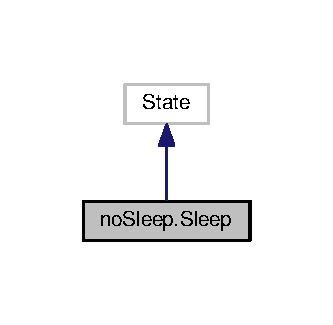
\includegraphics[width=160pt]{classnoSleep_1_1Sleep__inherit__graph}
\end{center}
\end{figure}


Collaboration diagram for no\+Sleep.\+Sleep\+:\nopagebreak
\begin{figure}[H]
\begin{center}
\leavevmode
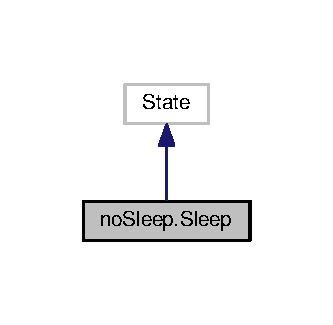
\includegraphics[width=160pt]{classnoSleep_1_1Sleep__coll__graph}
\end{center}
\end{figure}
\subsection*{Public Member Functions}
\begin{DoxyCompactItemize}
\item 
def \hyperlink{classnoSleep_1_1Sleep_a5e503c196ce370db0858f3bc1f26a5e4}{\+\_\+\+\_\+init\+\_\+\+\_\+} (self)
\item 
def \hyperlink{classnoSleep_1_1Sleep_a1766a04aa16120154e8f72359d9603a3}{execute} (self, userdata)
\end{DoxyCompactItemize}
\subsection*{Public Attributes}
\begin{DoxyCompactItemize}
\item 
\hyperlink{classnoSleep_1_1Sleep_a376ccc728046a13c934edeab50e6e56d}{rate}
\end{DoxyCompactItemize}
\subsection*{Static Public Attributes}
\begin{DoxyCompactItemize}
\item 
\hyperlink{classnoSleep_1_1Sleep_a54db281a8ae734c31979bfcb6e48dc74}{position} = rooms.\+get\+\_\+room\+\_\+position(\char`\"{}Home\char`\"{})
\end{DoxyCompactItemize}


\subsection{Detailed Description}
\begin{DoxyVerb}It defines the SLEEP state where the robot sleeps for a random period of time.
Then it makes a request to the move_base action server to go to the home location.
Finally it returns in the NORMAL state\end{DoxyVerb}
 

\subsection{Constructor \& Destructor Documentation}
\index{no\+Sleep\+::\+Sleep@{no\+Sleep\+::\+Sleep}!\+\_\+\+\_\+init\+\_\+\+\_\+@{\+\_\+\+\_\+init\+\_\+\+\_\+}}
\index{\+\_\+\+\_\+init\+\_\+\+\_\+@{\+\_\+\+\_\+init\+\_\+\+\_\+}!no\+Sleep\+::\+Sleep@{no\+Sleep\+::\+Sleep}}
\subsubsection[{\texorpdfstring{\+\_\+\+\_\+init\+\_\+\+\_\+(self)}{__init__(self)}}]{\setlength{\rightskip}{0pt plus 5cm}def no\+Sleep.\+Sleep.\+\_\+\+\_\+init\+\_\+\+\_\+ (
\begin{DoxyParamCaption}
\item[{}]{self}
\end{DoxyParamCaption}
)}\hypertarget{classnoSleep_1_1Sleep_a5e503c196ce370db0858f3bc1f26a5e4}{}\label{classnoSleep_1_1Sleep_a5e503c196ce370db0858f3bc1f26a5e4}
\begin{DoxyVerb}It defines the SLEEP state where the robot sleeps for a random period of time.
Then it makes a request to the move_base action server to go to the home location.
Finally it returns in the NORMAL state\end{DoxyVerb}
 

\subsection{Member Function Documentation}
\index{no\+Sleep\+::\+Sleep@{no\+Sleep\+::\+Sleep}!execute@{execute}}
\index{execute@{execute}!no\+Sleep\+::\+Sleep@{no\+Sleep\+::\+Sleep}}
\subsubsection[{\texorpdfstring{execute(self, userdata)}{execute(self, userdata)}}]{\setlength{\rightskip}{0pt plus 5cm}def no\+Sleep.\+Sleep.\+execute (
\begin{DoxyParamCaption}
\item[{}]{self, }
\item[{}]{userdata}
\end{DoxyParamCaption}
)}\hypertarget{classnoSleep_1_1Sleep_a1766a04aa16120154e8f72359d9603a3}{}\label{classnoSleep_1_1Sleep_a1766a04aa16120154e8f72359d9603a3}


\subsection{Member Data Documentation}
\index{no\+Sleep\+::\+Sleep@{no\+Sleep\+::\+Sleep}!position@{position}}
\index{position@{position}!no\+Sleep\+::\+Sleep@{no\+Sleep\+::\+Sleep}}
\subsubsection[{\texorpdfstring{position}{position}}]{\setlength{\rightskip}{0pt plus 5cm}no\+Sleep.\+Sleep.\+position = rooms.\+get\+\_\+room\+\_\+position(\char`\"{}Home\char`\"{})\hspace{0.3cm}{\ttfamily [static]}}\hypertarget{classnoSleep_1_1Sleep_a54db281a8ae734c31979bfcb6e48dc74}{}\label{classnoSleep_1_1Sleep_a54db281a8ae734c31979bfcb6e48dc74}
\index{no\+Sleep\+::\+Sleep@{no\+Sleep\+::\+Sleep}!rate@{rate}}
\index{rate@{rate}!no\+Sleep\+::\+Sleep@{no\+Sleep\+::\+Sleep}}
\subsubsection[{\texorpdfstring{rate}{rate}}]{\setlength{\rightskip}{0pt plus 5cm}no\+Sleep.\+Sleep.\+rate}\hypertarget{classnoSleep_1_1Sleep_a376ccc728046a13c934edeab50e6e56d}{}\label{classnoSleep_1_1Sleep_a376ccc728046a13c934edeab50e6e56d}


The documentation for this class was generated from the following file\+:\begin{DoxyCompactItemize}
\item 
/home/francescotesta/experimental\+\_\+ws/src/final\+\_\+assignment/scripts/\hyperlink{noSleep_8py}{no\+Sleep.\+py}\end{DoxyCompactItemize}

\hypertarget{classcommandManager_1_1Sleep}{}\section{command\+Manager.\+Sleep Class Reference}
\label{classcommandManager_1_1Sleep}\index{command\+Manager.\+Sleep@{command\+Manager.\+Sleep}}


Inheritance diagram for command\+Manager.\+Sleep\+:\nopagebreak
\begin{figure}[H]
\begin{center}
\leavevmode
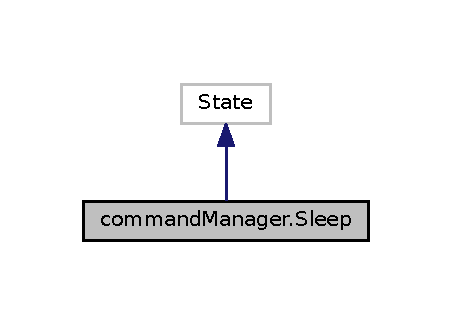
\includegraphics[width=217pt]{classcommandManager_1_1Sleep__inherit__graph}
\end{center}
\end{figure}


Collaboration diagram for command\+Manager.\+Sleep\+:\nopagebreak
\begin{figure}[H]
\begin{center}
\leavevmode
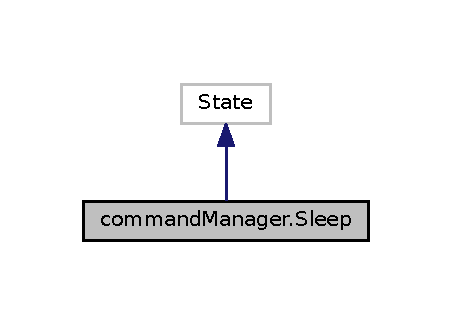
\includegraphics[width=217pt]{classcommandManager_1_1Sleep__coll__graph}
\end{center}
\end{figure}
\subsection*{Public Member Functions}
\begin{DoxyCompactItemize}
\item 
def \hyperlink{classcommandManager_1_1Sleep_aa31bb1cc360e9bb1d723eaf953295268}{\+\_\+\+\_\+init\+\_\+\+\_\+} (self)
\item 
def \hyperlink{classcommandManager_1_1Sleep_a01a1b33499ec3c862bed42a6258b0f12}{execute} (self, userdata)
\end{DoxyCompactItemize}
\subsection*{Public Attributes}
\begin{DoxyCompactItemize}
\item 
\hyperlink{classcommandManager_1_1Sleep_ad1bca2bd2c57109d92089b82fafe23c1}{rate}
\end{DoxyCompactItemize}
\subsection*{Static Public Attributes}
\begin{DoxyCompactItemize}
\item 
\hyperlink{classcommandManager_1_1Sleep_ab64714b4c7c4b5a8824986a8e7af976e}{position} = rooms.\+get\+\_\+room\+\_\+position(\char`\"{}Home\char`\"{})
\end{DoxyCompactItemize}


\subsection{Detailed Description}
\begin{DoxyVerb}It defines the SLEEP state where the robot sleeps for a random period of time.
Then it makes a request to the move_base action server to go to the home location.
Finally it returns in the NORMAL state\end{DoxyVerb}
 

\subsection{Constructor \& Destructor Documentation}
\index{command\+Manager\+::\+Sleep@{command\+Manager\+::\+Sleep}!\+\_\+\+\_\+init\+\_\+\+\_\+@{\+\_\+\+\_\+init\+\_\+\+\_\+}}
\index{\+\_\+\+\_\+init\+\_\+\+\_\+@{\+\_\+\+\_\+init\+\_\+\+\_\+}!command\+Manager\+::\+Sleep@{command\+Manager\+::\+Sleep}}
\subsubsection[{\texorpdfstring{\+\_\+\+\_\+init\+\_\+\+\_\+(self)}{__init__(self)}}]{\setlength{\rightskip}{0pt plus 5cm}def command\+Manager.\+Sleep.\+\_\+\+\_\+init\+\_\+\+\_\+ (
\begin{DoxyParamCaption}
\item[{}]{self}
\end{DoxyParamCaption}
)}\hypertarget{classcommandManager_1_1Sleep_aa31bb1cc360e9bb1d723eaf953295268}{}\label{classcommandManager_1_1Sleep_aa31bb1cc360e9bb1d723eaf953295268}
\begin{DoxyVerb}It defines the SLEEP state where the robot sleeps for a random period of time.
Then it makes a request to the move_base action server to go to the home location.
Finally it returns in the NORMAL state\end{DoxyVerb}
 

\subsection{Member Function Documentation}
\index{command\+Manager\+::\+Sleep@{command\+Manager\+::\+Sleep}!execute@{execute}}
\index{execute@{execute}!command\+Manager\+::\+Sleep@{command\+Manager\+::\+Sleep}}
\subsubsection[{\texorpdfstring{execute(self, userdata)}{execute(self, userdata)}}]{\setlength{\rightskip}{0pt plus 5cm}def command\+Manager.\+Sleep.\+execute (
\begin{DoxyParamCaption}
\item[{}]{self, }
\item[{}]{userdata}
\end{DoxyParamCaption}
)}\hypertarget{classcommandManager_1_1Sleep_a01a1b33499ec3c862bed42a6258b0f12}{}\label{classcommandManager_1_1Sleep_a01a1b33499ec3c862bed42a6258b0f12}


\subsection{Member Data Documentation}
\index{command\+Manager\+::\+Sleep@{command\+Manager\+::\+Sleep}!position@{position}}
\index{position@{position}!command\+Manager\+::\+Sleep@{command\+Manager\+::\+Sleep}}
\subsubsection[{\texorpdfstring{position}{position}}]{\setlength{\rightskip}{0pt plus 5cm}command\+Manager.\+Sleep.\+position = rooms.\+get\+\_\+room\+\_\+position(\char`\"{}Home\char`\"{})\hspace{0.3cm}{\ttfamily [static]}}\hypertarget{classcommandManager_1_1Sleep_ab64714b4c7c4b5a8824986a8e7af976e}{}\label{classcommandManager_1_1Sleep_ab64714b4c7c4b5a8824986a8e7af976e}
\index{command\+Manager\+::\+Sleep@{command\+Manager\+::\+Sleep}!rate@{rate}}
\index{rate@{rate}!command\+Manager\+::\+Sleep@{command\+Manager\+::\+Sleep}}
\subsubsection[{\texorpdfstring{rate}{rate}}]{\setlength{\rightskip}{0pt plus 5cm}command\+Manager.\+Sleep.\+rate}\hypertarget{classcommandManager_1_1Sleep_ad1bca2bd2c57109d92089b82fafe23c1}{}\label{classcommandManager_1_1Sleep_ad1bca2bd2c57109d92089b82fafe23c1}


The documentation for this class was generated from the following file\+:\begin{DoxyCompactItemize}
\item 
/home/francescotesta/experimental\+\_\+ws/src/final\+\_\+assignment/scripts/\hyperlink{commandManager_8py}{command\+Manager.\+py}\end{DoxyCompactItemize}

\hypertarget{classnoSleep_1_1Track}{}\section{no\+Sleep.\+Track Class Reference}
\label{classnoSleep_1_1Track}\index{no\+Sleep.\+Track@{no\+Sleep.\+Track}}


Inheritance diagram for no\+Sleep.\+Track\+:\nopagebreak
\begin{figure}[H]
\begin{center}
\leavevmode
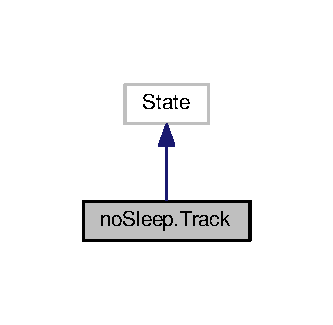
\includegraphics[width=160pt]{classnoSleep_1_1Track__inherit__graph}
\end{center}
\end{figure}


Collaboration diagram for no\+Sleep.\+Track\+:\nopagebreak
\begin{figure}[H]
\begin{center}
\leavevmode
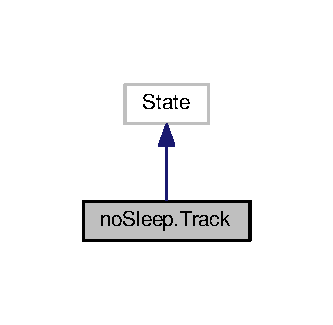
\includegraphics[width=160pt]{classnoSleep_1_1Track__coll__graph}
\end{center}
\end{figure}
\subsection*{Public Member Functions}
\begin{DoxyCompactItemize}
\item 
def \hyperlink{classnoSleep_1_1Track_a9af26ff426231cb9c1bc6e5395cf6ec5}{\+\_\+\+\_\+init\+\_\+\+\_\+} (self)
\item 
def \hyperlink{classnoSleep_1_1Track_aa6bbc699fd4253fec111652d41221990}{execute} (self, userdata)
\end{DoxyCompactItemize}
\subsection*{Static Public Attributes}
\begin{DoxyCompactItemize}
\item 
\hyperlink{classnoSleep_1_1Track_a858198e9049836b190bd6920cb40d482}{goal} = track\+Ball\+Goal()
\item 
\hyperlink{classnoSleep_1_1Track_a9656da60a353880af15789af38d37944}{color}
\item 
\hyperlink{classnoSleep_1_1Track_aa81312a09b71e383923eea00179b2330}{track\+Client} = actionlib.\+Simple\+Action\+Client(\textquotesingle{}track\+Action\textquotesingle{},track\+Ball\+Action)
\item 
\hyperlink{classnoSleep_1_1Track_ab87d8de18ccaf82e3d818c8c3241a220}{wait} = track\+Client.\+wait\+\_\+for\+\_\+result()
\item 
\hyperlink{classnoSleep_1_1Track_ab23617bf485f7d5bc2c03e0b6b17017f}{result} = track\+Client.\+get\+\_\+result()
\end{DoxyCompactItemize}


\subsection{Detailed Description}
\begin{DoxyVerb}Class that defines the TRACK state. 
 It send the detected color room to the track action server in order ot reach it. 
 Then sotores the location of the room found \end{DoxyVerb}
 

\subsection{Constructor \& Destructor Documentation}
\index{no\+Sleep\+::\+Track@{no\+Sleep\+::\+Track}!\+\_\+\+\_\+init\+\_\+\+\_\+@{\+\_\+\+\_\+init\+\_\+\+\_\+}}
\index{\+\_\+\+\_\+init\+\_\+\+\_\+@{\+\_\+\+\_\+init\+\_\+\+\_\+}!no\+Sleep\+::\+Track@{no\+Sleep\+::\+Track}}
\subsubsection[{\texorpdfstring{\+\_\+\+\_\+init\+\_\+\+\_\+(self)}{__init__(self)}}]{\setlength{\rightskip}{0pt plus 5cm}def no\+Sleep.\+Track.\+\_\+\+\_\+init\+\_\+\+\_\+ (
\begin{DoxyParamCaption}
\item[{}]{self}
\end{DoxyParamCaption}
)}\hypertarget{classnoSleep_1_1Track_a9af26ff426231cb9c1bc6e5395cf6ec5}{}\label{classnoSleep_1_1Track_a9af26ff426231cb9c1bc6e5395cf6ec5}
\begin{DoxyVerb}Class that defines the TRACK state. 
 It send the detected color room to the track action server in order ot reach it. 
 Then sotores the location of the room found \end{DoxyVerb}
 

\subsection{Member Function Documentation}
\index{no\+Sleep\+::\+Track@{no\+Sleep\+::\+Track}!execute@{execute}}
\index{execute@{execute}!no\+Sleep\+::\+Track@{no\+Sleep\+::\+Track}}
\subsubsection[{\texorpdfstring{execute(self, userdata)}{execute(self, userdata)}}]{\setlength{\rightskip}{0pt plus 5cm}def no\+Sleep.\+Track.\+execute (
\begin{DoxyParamCaption}
\item[{}]{self, }
\item[{}]{userdata}
\end{DoxyParamCaption}
)}\hypertarget{classnoSleep_1_1Track_aa6bbc699fd4253fec111652d41221990}{}\label{classnoSleep_1_1Track_aa6bbc699fd4253fec111652d41221990}


\subsection{Member Data Documentation}
\index{no\+Sleep\+::\+Track@{no\+Sleep\+::\+Track}!color@{color}}
\index{color@{color}!no\+Sleep\+::\+Track@{no\+Sleep\+::\+Track}}
\subsubsection[{\texorpdfstring{color}{color}}]{\setlength{\rightskip}{0pt plus 5cm}no\+Sleep.\+Track.\+color\hspace{0.3cm}{\ttfamily [static]}}\hypertarget{classnoSleep_1_1Track_a9656da60a353880af15789af38d37944}{}\label{classnoSleep_1_1Track_a9656da60a353880af15789af38d37944}
\index{no\+Sleep\+::\+Track@{no\+Sleep\+::\+Track}!goal@{goal}}
\index{goal@{goal}!no\+Sleep\+::\+Track@{no\+Sleep\+::\+Track}}
\subsubsection[{\texorpdfstring{goal}{goal}}]{\setlength{\rightskip}{0pt plus 5cm}no\+Sleep.\+Track.\+goal = track\+Ball\+Goal()\hspace{0.3cm}{\ttfamily [static]}}\hypertarget{classnoSleep_1_1Track_a858198e9049836b190bd6920cb40d482}{}\label{classnoSleep_1_1Track_a858198e9049836b190bd6920cb40d482}
\index{no\+Sleep\+::\+Track@{no\+Sleep\+::\+Track}!result@{result}}
\index{result@{result}!no\+Sleep\+::\+Track@{no\+Sleep\+::\+Track}}
\subsubsection[{\texorpdfstring{result}{result}}]{\setlength{\rightskip}{0pt plus 5cm}no\+Sleep.\+Track.\+result = track\+Client.\+get\+\_\+result()\hspace{0.3cm}{\ttfamily [static]}}\hypertarget{classnoSleep_1_1Track_ab23617bf485f7d5bc2c03e0b6b17017f}{}\label{classnoSleep_1_1Track_ab23617bf485f7d5bc2c03e0b6b17017f}
\index{no\+Sleep\+::\+Track@{no\+Sleep\+::\+Track}!track\+Client@{track\+Client}}
\index{track\+Client@{track\+Client}!no\+Sleep\+::\+Track@{no\+Sleep\+::\+Track}}
\subsubsection[{\texorpdfstring{track\+Client}{trackClient}}]{\setlength{\rightskip}{0pt plus 5cm}no\+Sleep.\+Track.\+track\+Client = actionlib.\+Simple\+Action\+Client(\textquotesingle{}track\+Action\textquotesingle{},track\+Ball\+Action)\hspace{0.3cm}{\ttfamily [static]}}\hypertarget{classnoSleep_1_1Track_aa81312a09b71e383923eea00179b2330}{}\label{classnoSleep_1_1Track_aa81312a09b71e383923eea00179b2330}
\index{no\+Sleep\+::\+Track@{no\+Sleep\+::\+Track}!wait@{wait}}
\index{wait@{wait}!no\+Sleep\+::\+Track@{no\+Sleep\+::\+Track}}
\subsubsection[{\texorpdfstring{wait}{wait}}]{\setlength{\rightskip}{0pt plus 5cm}no\+Sleep.\+Track.\+wait = track\+Client.\+wait\+\_\+for\+\_\+result()\hspace{0.3cm}{\ttfamily [static]}}\hypertarget{classnoSleep_1_1Track_ab87d8de18ccaf82e3d818c8c3241a220}{}\label{classnoSleep_1_1Track_ab87d8de18ccaf82e3d818c8c3241a220}


The documentation for this class was generated from the following file\+:\begin{DoxyCompactItemize}
\item 
/home/francescotesta/experimental\+\_\+ws/src/final\+\_\+assignment/scripts/\hyperlink{noSleep_8py}{no\+Sleep.\+py}\end{DoxyCompactItemize}

\hypertarget{classcommandManager_1_1Track}{}\section{command\+Manager.\+Track Class Reference}
\label{classcommandManager_1_1Track}\index{command\+Manager.\+Track@{command\+Manager.\+Track}}


Inheritance diagram for command\+Manager.\+Track\+:\nopagebreak
\begin{figure}[H]
\begin{center}
\leavevmode
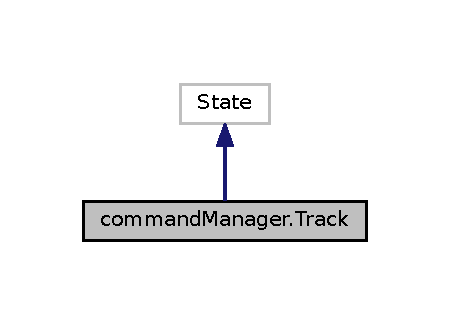
\includegraphics[width=216pt]{classcommandManager_1_1Track__inherit__graph}
\end{center}
\end{figure}


Collaboration diagram for command\+Manager.\+Track\+:\nopagebreak
\begin{figure}[H]
\begin{center}
\leavevmode
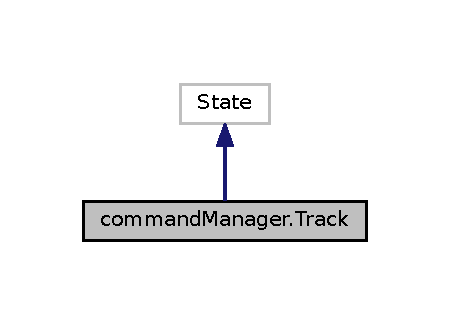
\includegraphics[width=216pt]{classcommandManager_1_1Track__coll__graph}
\end{center}
\end{figure}
\subsection*{Public Member Functions}
\begin{DoxyCompactItemize}
\item 
def \hyperlink{classcommandManager_1_1Track_af204111942c1cc2b65ff7b68a74c2420}{\+\_\+\+\_\+init\+\_\+\+\_\+} (self)
\item 
def \hyperlink{classcommandManager_1_1Track_a58dac1ae26362ef259735b950e35e237}{execute} (self, userdata)
\end{DoxyCompactItemize}
\subsection*{Static Public Attributes}
\begin{DoxyCompactItemize}
\item 
\hyperlink{classcommandManager_1_1Track_aaf31135bbe355747fc8e8ebbfa9ea7c3}{goal} = track\+Ball\+Goal()
\item 
\hyperlink{classcommandManager_1_1Track_acaaf54b9a806780342efd702c43ca892}{color}
\item 
\hyperlink{classcommandManager_1_1Track_a4a57e4e548d9213c4623f5d528753b1f}{track\+Client} = actionlib.\+Simple\+Action\+Client(\textquotesingle{}track\+Action\textquotesingle{},track\+Ball\+Action)
\item 
bool \hyperlink{classcommandManager_1_1Track_afb7ce9aacf03e990b6ecca9c7641caeb}{N\+E\+W\+\_\+\+R\+O\+OM} = False
\item 
\hyperlink{classcommandManager_1_1Track_a8f86bbb5fd3d92749c09d5e876a1d1a6}{wait} = track\+Client.\+wait\+\_\+for\+\_\+result()
\item 
\hyperlink{classcommandManager_1_1Track_aa66fb1baab2433c729df0919ba0989a7}{result} = track\+Client.\+get\+\_\+result()
\item 
bool \hyperlink{classcommandManager_1_1Track_af7f0cd8d298db357c98855ffd93eff1b}{F\+I\+N\+D\+\_\+\+M\+O\+DE} = False
\end{DoxyCompactItemize}


\subsection{Detailed Description}
\begin{DoxyVerb}Class that defines the PLAY state. 
 It move the robot in X Y location and then asks to go back to the user.\end{DoxyVerb}
 

\subsection{Constructor \& Destructor Documentation}
\index{command\+Manager\+::\+Track@{command\+Manager\+::\+Track}!\+\_\+\+\_\+init\+\_\+\+\_\+@{\+\_\+\+\_\+init\+\_\+\+\_\+}}
\index{\+\_\+\+\_\+init\+\_\+\+\_\+@{\+\_\+\+\_\+init\+\_\+\+\_\+}!command\+Manager\+::\+Track@{command\+Manager\+::\+Track}}
\subsubsection[{\texorpdfstring{\+\_\+\+\_\+init\+\_\+\+\_\+(self)}{__init__(self)}}]{\setlength{\rightskip}{0pt plus 5cm}def command\+Manager.\+Track.\+\_\+\+\_\+init\+\_\+\+\_\+ (
\begin{DoxyParamCaption}
\item[{}]{self}
\end{DoxyParamCaption}
)}\hypertarget{classcommandManager_1_1Track_af204111942c1cc2b65ff7b68a74c2420}{}\label{classcommandManager_1_1Track_af204111942c1cc2b65ff7b68a74c2420}
\begin{DoxyVerb}Class that defines the PLAY state. 
 It move the robot in X Y location and then asks to go back to the user.\end{DoxyVerb}
 

\subsection{Member Function Documentation}
\index{command\+Manager\+::\+Track@{command\+Manager\+::\+Track}!execute@{execute}}
\index{execute@{execute}!command\+Manager\+::\+Track@{command\+Manager\+::\+Track}}
\subsubsection[{\texorpdfstring{execute(self, userdata)}{execute(self, userdata)}}]{\setlength{\rightskip}{0pt plus 5cm}def command\+Manager.\+Track.\+execute (
\begin{DoxyParamCaption}
\item[{}]{self, }
\item[{}]{userdata}
\end{DoxyParamCaption}
)}\hypertarget{classcommandManager_1_1Track_a58dac1ae26362ef259735b950e35e237}{}\label{classcommandManager_1_1Track_a58dac1ae26362ef259735b950e35e237}


\subsection{Member Data Documentation}
\index{command\+Manager\+::\+Track@{command\+Manager\+::\+Track}!color@{color}}
\index{color@{color}!command\+Manager\+::\+Track@{command\+Manager\+::\+Track}}
\subsubsection[{\texorpdfstring{color}{color}}]{\setlength{\rightskip}{0pt plus 5cm}command\+Manager.\+Track.\+color\hspace{0.3cm}{\ttfamily [static]}}\hypertarget{classcommandManager_1_1Track_acaaf54b9a806780342efd702c43ca892}{}\label{classcommandManager_1_1Track_acaaf54b9a806780342efd702c43ca892}
\index{command\+Manager\+::\+Track@{command\+Manager\+::\+Track}!F\+I\+N\+D\+\_\+\+M\+O\+DE@{F\+I\+N\+D\+\_\+\+M\+O\+DE}}
\index{F\+I\+N\+D\+\_\+\+M\+O\+DE@{F\+I\+N\+D\+\_\+\+M\+O\+DE}!command\+Manager\+::\+Track@{command\+Manager\+::\+Track}}
\subsubsection[{\texorpdfstring{F\+I\+N\+D\+\_\+\+M\+O\+DE}{FIND_MODE}}]{\setlength{\rightskip}{0pt plus 5cm}bool command\+Manager.\+Track.\+F\+I\+N\+D\+\_\+\+M\+O\+DE = False\hspace{0.3cm}{\ttfamily [static]}}\hypertarget{classcommandManager_1_1Track_af7f0cd8d298db357c98855ffd93eff1b}{}\label{classcommandManager_1_1Track_af7f0cd8d298db357c98855ffd93eff1b}
\index{command\+Manager\+::\+Track@{command\+Manager\+::\+Track}!goal@{goal}}
\index{goal@{goal}!command\+Manager\+::\+Track@{command\+Manager\+::\+Track}}
\subsubsection[{\texorpdfstring{goal}{goal}}]{\setlength{\rightskip}{0pt plus 5cm}command\+Manager.\+Track.\+goal = track\+Ball\+Goal()\hspace{0.3cm}{\ttfamily [static]}}\hypertarget{classcommandManager_1_1Track_aaf31135bbe355747fc8e8ebbfa9ea7c3}{}\label{classcommandManager_1_1Track_aaf31135bbe355747fc8e8ebbfa9ea7c3}
\index{command\+Manager\+::\+Track@{command\+Manager\+::\+Track}!N\+E\+W\+\_\+\+R\+O\+OM@{N\+E\+W\+\_\+\+R\+O\+OM}}
\index{N\+E\+W\+\_\+\+R\+O\+OM@{N\+E\+W\+\_\+\+R\+O\+OM}!command\+Manager\+::\+Track@{command\+Manager\+::\+Track}}
\subsubsection[{\texorpdfstring{N\+E\+W\+\_\+\+R\+O\+OM}{NEW_ROOM}}]{\setlength{\rightskip}{0pt plus 5cm}bool command\+Manager.\+Track.\+N\+E\+W\+\_\+\+R\+O\+OM = False\hspace{0.3cm}{\ttfamily [static]}}\hypertarget{classcommandManager_1_1Track_afb7ce9aacf03e990b6ecca9c7641caeb}{}\label{classcommandManager_1_1Track_afb7ce9aacf03e990b6ecca9c7641caeb}
\index{command\+Manager\+::\+Track@{command\+Manager\+::\+Track}!result@{result}}
\index{result@{result}!command\+Manager\+::\+Track@{command\+Manager\+::\+Track}}
\subsubsection[{\texorpdfstring{result}{result}}]{\setlength{\rightskip}{0pt plus 5cm}command\+Manager.\+Track.\+result = track\+Client.\+get\+\_\+result()\hspace{0.3cm}{\ttfamily [static]}}\hypertarget{classcommandManager_1_1Track_aa66fb1baab2433c729df0919ba0989a7}{}\label{classcommandManager_1_1Track_aa66fb1baab2433c729df0919ba0989a7}
\index{command\+Manager\+::\+Track@{command\+Manager\+::\+Track}!track\+Client@{track\+Client}}
\index{track\+Client@{track\+Client}!command\+Manager\+::\+Track@{command\+Manager\+::\+Track}}
\subsubsection[{\texorpdfstring{track\+Client}{trackClient}}]{\setlength{\rightskip}{0pt plus 5cm}command\+Manager.\+Track.\+track\+Client = actionlib.\+Simple\+Action\+Client(\textquotesingle{}track\+Action\textquotesingle{},track\+Ball\+Action)\hspace{0.3cm}{\ttfamily [static]}}\hypertarget{classcommandManager_1_1Track_a4a57e4e548d9213c4623f5d528753b1f}{}\label{classcommandManager_1_1Track_a4a57e4e548d9213c4623f5d528753b1f}
\index{command\+Manager\+::\+Track@{command\+Manager\+::\+Track}!wait@{wait}}
\index{wait@{wait}!command\+Manager\+::\+Track@{command\+Manager\+::\+Track}}
\subsubsection[{\texorpdfstring{wait}{wait}}]{\setlength{\rightskip}{0pt plus 5cm}command\+Manager.\+Track.\+wait = track\+Client.\+wait\+\_\+for\+\_\+result()\hspace{0.3cm}{\ttfamily [static]}}\hypertarget{classcommandManager_1_1Track_a8f86bbb5fd3d92749c09d5e876a1d1a6}{}\label{classcommandManager_1_1Track_a8f86bbb5fd3d92749c09d5e876a1d1a6}


The documentation for this class was generated from the following file\+:\begin{DoxyCompactItemize}
\item 
/home/francescotesta/experimental\+\_\+ws/src/final\+\_\+assignment/scripts/\hyperlink{commandManager_8py}{command\+Manager.\+py}\end{DoxyCompactItemize}

\hypertarget{classtrack_1_1TrackAction}{}\section{track.\+Track\+Action Class Reference}
\label{classtrack_1_1TrackAction}\index{track.\+Track\+Action@{track.\+Track\+Action}}


Class that implements the action server for tracking the ball.  




Inheritance diagram for track.\+Track\+Action\+:\nopagebreak
\begin{figure}[H]
\begin{center}
\leavevmode
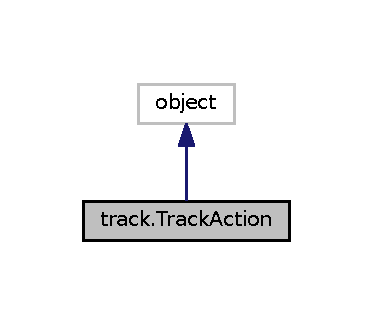
\includegraphics[width=179pt]{classtrack_1_1TrackAction__inherit__graph}
\end{center}
\end{figure}


Collaboration diagram for track.\+Track\+Action\+:\nopagebreak
\begin{figure}[H]
\begin{center}
\leavevmode
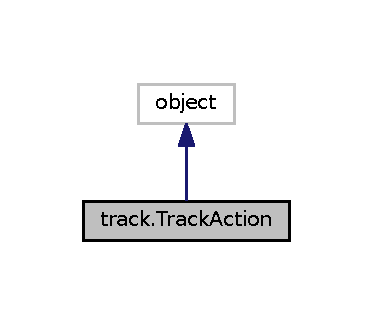
\includegraphics[width=179pt]{classtrack_1_1TrackAction__coll__graph}
\end{center}
\end{figure}
\subsection*{Public Member Functions}
\begin{DoxyCompactItemize}
\item 
def \hyperlink{classtrack_1_1TrackAction_ad71d2ce7ecd91c384219ada7e8ed74e3}{\+\_\+\+\_\+init\+\_\+\+\_\+} (self, name)
\item 
def \hyperlink{classtrack_1_1TrackAction_a3b41ed0eb7a403459469c27dd63a2392}{reach\+\_\+ball} (self, ros\+\_\+image)
\begin{DoxyCompactList}\small\item\em Callback function of the camera subscriber which computes the velocities to apply to the robot untill it reaches the ball. \end{DoxyCompactList}\item 
def \hyperlink{classtrack_1_1TrackAction_a1d41a25e35227ab25323a95eeb9a4bb2}{track} (self, goal)
\begin{DoxyCompactList}\small\item\em Action server routine function. \end{DoxyCompactList}\end{DoxyCompactItemize}
\subsection*{Public Attributes}
\begin{DoxyCompactItemize}
\item 
\hyperlink{classtrack_1_1TrackAction_abba894c7d22403050003dc50f5d79bba}{color}
\begin{DoxyCompactList}\small\item\em direct conversion to C\+V2 \#\#\#\# \end{DoxyCompactList}\end{DoxyCompactItemize}
\subsection*{Static Public Attributes}
\begin{DoxyCompactItemize}
\item 
\hyperlink{classtrack_1_1TrackAction_abb57579f14aa39d1cc0f4379382390a6}{action\+Name}
\begin{DoxyCompactList}\small\item\em Name of the action server. \end{DoxyCompactList}\item 
\hyperlink{classtrack_1_1TrackAction_ae1870a4393e99629a3835f563374152e}{act\+\_\+s}
\item 
\hyperlink{classtrack_1_1TrackAction_a3d89a5a6bf3daf63df4b690e4c9a84a8}{track}
\item 
\hyperlink{classtrack_1_1TrackAction_aeb30f796983b2999ad62d71535795668}{auto\+\_\+start}
\item 
\hyperlink{classtrack_1_1TrackAction_acce0064c9d83a91f00d92a854014cdf5}{feedback}
\item 
\hyperlink{classtrack_1_1TrackAction_ae62bfb3233b566df94fde636d8d26877}{result}
\item 
\hyperlink{classtrack_1_1TrackAction_a8c79189ba62cf316bffaa4c00b0320fe}{success}
\begin{DoxyCompactList}\small\item\em Flag that notifies that the robot has reached the ball correctly. \end{DoxyCompactList}\item 
\hyperlink{classtrack_1_1TrackAction_aabc16f100d1f260d6712d8d74e055fda}{unfound\+\_\+ball\+\_\+counter}
\begin{DoxyCompactList}\small\item\em Variables that counts how many times the robot was not able to detect the ball again. \end{DoxyCompactList}\item 
\hyperlink{classtrack_1_1TrackAction_a4fac0918d826dc6cbf110784c8fcda99}{abort}
\begin{DoxyCompactList}\small\item\em Flag that notifies aborting mission since the robot was not able to detect the ball. \end{DoxyCompactList}\item 
\hyperlink{classtrack_1_1TrackAction_a4cbc03d130bcf2203bc68f37d02dc4c5}{sub\+\_\+odom} = rospy.\+Subscriber(\textquotesingle{}odom\textquotesingle{}, Odometry, \hyperlink{namespacetrack_ac547a00259cf9bddfb37b60063740e8d}{clbk\+\_\+odom})
\begin{DoxyCompactList}\small\item\em Odom subcriber to get and save the robot position and send them back to the \hyperlink{namespacecommandManager}{command\+Manager}. \end{DoxyCompactList}\item 
\hyperlink{classtrack_1_1TrackAction_af6105c2cad0d325296213d7c03c4fb6e}{vel\+\_\+pub}
\begin{DoxyCompactList}\small\item\em Publisher to the cmd\+\_\+vel topic in order to move the robot. \end{DoxyCompactList}\item 
\hyperlink{classtrack_1_1TrackAction_aabd955eb5b74ee508ba27bf6db4129e2}{Twist}
\item 
\hyperlink{classtrack_1_1TrackAction_a47112fa77bb24c45494449d781bd35c4}{queue\+\_\+size}
\item 
\hyperlink{classtrack_1_1TrackAction_a71b1a13ec7fb0ba79d6f34416b7d54e1}{camera\+\_\+sub} = rospy.\+Subscriber(\char`\"{}camera1/image\+\_\+raw/compressed\char`\"{}, Compressed\+Image, self.\+reach\+\_\+ball, \hyperlink{classtrack_1_1TrackAction_a47112fa77bb24c45494449d781bd35c4}{queue\+\_\+size}=1)
\begin{DoxyCompactList}\small\item\em Subscriber to camera1 in order to recive and handle the images. \end{DoxyCompactList}\item 
\hyperlink{classtrack_1_1TrackAction_a56031d0f135cf2d2f7c950325059f7bd}{state}
\end{DoxyCompactItemize}


\subsection{Detailed Description}
Class that implements the action server for tracking the ball. 

\subsection{Constructor \& Destructor Documentation}
\index{track\+::\+Track\+Action@{track\+::\+Track\+Action}!\+\_\+\+\_\+init\+\_\+\+\_\+@{\+\_\+\+\_\+init\+\_\+\+\_\+}}
\index{\+\_\+\+\_\+init\+\_\+\+\_\+@{\+\_\+\+\_\+init\+\_\+\+\_\+}!track\+::\+Track\+Action@{track\+::\+Track\+Action}}
\subsubsection[{\texorpdfstring{\+\_\+\+\_\+init\+\_\+\+\_\+(self, name)}{__init__(self, name)}}]{\setlength{\rightskip}{0pt plus 5cm}def track.\+Track\+Action.\+\_\+\+\_\+init\+\_\+\+\_\+ (
\begin{DoxyParamCaption}
\item[{}]{self, }
\item[{}]{name}
\end{DoxyParamCaption}
)}\hypertarget{classtrack_1_1TrackAction_ad71d2ce7ecd91c384219ada7e8ed74e3}{}\label{classtrack_1_1TrackAction_ad71d2ce7ecd91c384219ada7e8ed74e3}


\subsection{Member Function Documentation}
\index{track\+::\+Track\+Action@{track\+::\+Track\+Action}!reach\+\_\+ball@{reach\+\_\+ball}}
\index{reach\+\_\+ball@{reach\+\_\+ball}!track\+::\+Track\+Action@{track\+::\+Track\+Action}}
\subsubsection[{\texorpdfstring{reach\+\_\+ball(self, ros\+\_\+image)}{reach_ball(self, ros_image)}}]{\setlength{\rightskip}{0pt plus 5cm}def track.\+Track\+Action.\+reach\+\_\+ball (
\begin{DoxyParamCaption}
\item[{}]{self, }
\item[{}]{ros\+\_\+image}
\end{DoxyParamCaption}
)}\hypertarget{classtrack_1_1TrackAction_a3b41ed0eb7a403459469c27dd63a2392}{}\label{classtrack_1_1TrackAction_a3b41ed0eb7a403459469c27dd63a2392}


Callback function of the camera subscriber which computes the velocities to apply to the robot untill it reaches the ball. 


\begin{DoxyParams}{Parameters}
{\em ros\+\_\+image} & is the image decompressed and converted in Opend\+Cv \\
\hline
\end{DoxyParams}
\index{track\+::\+Track\+Action@{track\+::\+Track\+Action}!track@{track}}
\index{track@{track}!track\+::\+Track\+Action@{track\+::\+Track\+Action}}
\subsubsection[{\texorpdfstring{track(self, goal)}{track(self, goal)}}]{\setlength{\rightskip}{0pt plus 5cm}def track.\+Track\+Action.\+track (
\begin{DoxyParamCaption}
\item[{}]{self, }
\item[{}]{goal}
\end{DoxyParamCaption}
)}\hypertarget{classtrack_1_1TrackAction_a1d41a25e35227ab25323a95eeb9a4bb2}{}\label{classtrack_1_1TrackAction_a1d41a25e35227ab25323a95eeb9a4bb2}


Action server routine function. 


\begin{DoxyParams}{Parameters}
{\em goal} & Contains the color of the ball that has been detected \\
\hline
\end{DoxyParams}


\subsection{Member Data Documentation}
\index{track\+::\+Track\+Action@{track\+::\+Track\+Action}!abort@{abort}}
\index{abort@{abort}!track\+::\+Track\+Action@{track\+::\+Track\+Action}}
\subsubsection[{\texorpdfstring{abort}{abort}}]{\setlength{\rightskip}{0pt plus 5cm}track.\+Track\+Action.\+abort\hspace{0.3cm}{\ttfamily [static]}}\hypertarget{classtrack_1_1TrackAction_a4fac0918d826dc6cbf110784c8fcda99}{}\label{classtrack_1_1TrackAction_a4fac0918d826dc6cbf110784c8fcda99}


Flag that notifies aborting mission since the robot was not able to detect the ball. 

\index{track\+::\+Track\+Action@{track\+::\+Track\+Action}!act\+\_\+s@{act\+\_\+s}}
\index{act\+\_\+s@{act\+\_\+s}!track\+::\+Track\+Action@{track\+::\+Track\+Action}}
\subsubsection[{\texorpdfstring{act\+\_\+s}{act_s}}]{\setlength{\rightskip}{0pt plus 5cm}track.\+Track\+Action.\+act\+\_\+s\hspace{0.3cm}{\ttfamily [static]}}\hypertarget{classtrack_1_1TrackAction_ae1870a4393e99629a3835f563374152e}{}\label{classtrack_1_1TrackAction_ae1870a4393e99629a3835f563374152e}
\index{track\+::\+Track\+Action@{track\+::\+Track\+Action}!action\+Name@{action\+Name}}
\index{action\+Name@{action\+Name}!track\+::\+Track\+Action@{track\+::\+Track\+Action}}
\subsubsection[{\texorpdfstring{action\+Name}{actionName}}]{\setlength{\rightskip}{0pt plus 5cm}track.\+Track\+Action.\+action\+Name\hspace{0.3cm}{\ttfamily [static]}}\hypertarget{classtrack_1_1TrackAction_abb57579f14aa39d1cc0f4379382390a6}{}\label{classtrack_1_1TrackAction_abb57579f14aa39d1cc0f4379382390a6}


Name of the action server. 

\index{track\+::\+Track\+Action@{track\+::\+Track\+Action}!auto\+\_\+start@{auto\+\_\+start}}
\index{auto\+\_\+start@{auto\+\_\+start}!track\+::\+Track\+Action@{track\+::\+Track\+Action}}
\subsubsection[{\texorpdfstring{auto\+\_\+start}{auto_start}}]{\setlength{\rightskip}{0pt plus 5cm}track.\+Track\+Action.\+auto\+\_\+start\hspace{0.3cm}{\ttfamily [static]}}\hypertarget{classtrack_1_1TrackAction_aeb30f796983b2999ad62d71535795668}{}\label{classtrack_1_1TrackAction_aeb30f796983b2999ad62d71535795668}
\index{track\+::\+Track\+Action@{track\+::\+Track\+Action}!camera\+\_\+sub@{camera\+\_\+sub}}
\index{camera\+\_\+sub@{camera\+\_\+sub}!track\+::\+Track\+Action@{track\+::\+Track\+Action}}
\subsubsection[{\texorpdfstring{camera\+\_\+sub}{camera_sub}}]{\setlength{\rightskip}{0pt plus 5cm}track.\+Track\+Action.\+camera\+\_\+sub = rospy.\+Subscriber(\char`\"{}camera1/image\+\_\+raw/compressed\char`\"{}, Compressed\+Image, self.\+reach\+\_\+ball, {\bf queue\+\_\+size}=1)\hspace{0.3cm}{\ttfamily [static]}}\hypertarget{classtrack_1_1TrackAction_a71b1a13ec7fb0ba79d6f34416b7d54e1}{}\label{classtrack_1_1TrackAction_a71b1a13ec7fb0ba79d6f34416b7d54e1}


Subscriber to camera1 in order to recive and handle the images. 

\index{track\+::\+Track\+Action@{track\+::\+Track\+Action}!color@{color}}
\index{color@{color}!track\+::\+Track\+Action@{track\+::\+Track\+Action}}
\subsubsection[{\texorpdfstring{color}{color}}]{\setlength{\rightskip}{0pt plus 5cm}track.\+Track\+Action.\+color}\hypertarget{classtrack_1_1TrackAction_abba894c7d22403050003dc50f5d79bba}{}\label{classtrack_1_1TrackAction_abba894c7d22403050003dc50f5d79bba}


direct conversion to C\+V2 \#\#\#\# 

\index{track\+::\+Track\+Action@{track\+::\+Track\+Action}!feedback@{feedback}}
\index{feedback@{feedback}!track\+::\+Track\+Action@{track\+::\+Track\+Action}}
\subsubsection[{\texorpdfstring{feedback}{feedback}}]{\setlength{\rightskip}{0pt plus 5cm}track.\+Track\+Action.\+feedback\hspace{0.3cm}{\ttfamily [static]}}\hypertarget{classtrack_1_1TrackAction_acce0064c9d83a91f00d92a854014cdf5}{}\label{classtrack_1_1TrackAction_acce0064c9d83a91f00d92a854014cdf5}
\index{track\+::\+Track\+Action@{track\+::\+Track\+Action}!queue\+\_\+size@{queue\+\_\+size}}
\index{queue\+\_\+size@{queue\+\_\+size}!track\+::\+Track\+Action@{track\+::\+Track\+Action}}
\subsubsection[{\texorpdfstring{queue\+\_\+size}{queue_size}}]{\setlength{\rightskip}{0pt plus 5cm}track.\+Track\+Action.\+queue\+\_\+size\hspace{0.3cm}{\ttfamily [static]}}\hypertarget{classtrack_1_1TrackAction_a47112fa77bb24c45494449d781bd35c4}{}\label{classtrack_1_1TrackAction_a47112fa77bb24c45494449d781bd35c4}
\index{track\+::\+Track\+Action@{track\+::\+Track\+Action}!result@{result}}
\index{result@{result}!track\+::\+Track\+Action@{track\+::\+Track\+Action}}
\subsubsection[{\texorpdfstring{result}{result}}]{\setlength{\rightskip}{0pt plus 5cm}track.\+Track\+Action.\+result\hspace{0.3cm}{\ttfamily [static]}}\hypertarget{classtrack_1_1TrackAction_ae62bfb3233b566df94fde636d8d26877}{}\label{classtrack_1_1TrackAction_ae62bfb3233b566df94fde636d8d26877}
\index{track\+::\+Track\+Action@{track\+::\+Track\+Action}!state@{state}}
\index{state@{state}!track\+::\+Track\+Action@{track\+::\+Track\+Action}}
\subsubsection[{\texorpdfstring{state}{state}}]{\setlength{\rightskip}{0pt plus 5cm}track.\+Track\+Action.\+state\hspace{0.3cm}{\ttfamily [static]}}\hypertarget{classtrack_1_1TrackAction_a56031d0f135cf2d2f7c950325059f7bd}{}\label{classtrack_1_1TrackAction_a56031d0f135cf2d2f7c950325059f7bd}
\index{track\+::\+Track\+Action@{track\+::\+Track\+Action}!sub\+\_\+odom@{sub\+\_\+odom}}
\index{sub\+\_\+odom@{sub\+\_\+odom}!track\+::\+Track\+Action@{track\+::\+Track\+Action}}
\subsubsection[{\texorpdfstring{sub\+\_\+odom}{sub_odom}}]{\setlength{\rightskip}{0pt plus 5cm}track.\+Track\+Action.\+sub\+\_\+odom = rospy.\+Subscriber(\textquotesingle{}odom\textquotesingle{}, Odometry, {\bf clbk\+\_\+odom})\hspace{0.3cm}{\ttfamily [static]}}\hypertarget{classtrack_1_1TrackAction_a4cbc03d130bcf2203bc68f37d02dc4c5}{}\label{classtrack_1_1TrackAction_a4cbc03d130bcf2203bc68f37d02dc4c5}


Odom subcriber to get and save the robot position and send them back to the \hyperlink{namespacecommandManager}{command\+Manager}. 

\index{track\+::\+Track\+Action@{track\+::\+Track\+Action}!success@{success}}
\index{success@{success}!track\+::\+Track\+Action@{track\+::\+Track\+Action}}
\subsubsection[{\texorpdfstring{success}{success}}]{\setlength{\rightskip}{0pt plus 5cm}track.\+Track\+Action.\+success\hspace{0.3cm}{\ttfamily [static]}}\hypertarget{classtrack_1_1TrackAction_a8c79189ba62cf316bffaa4c00b0320fe}{}\label{classtrack_1_1TrackAction_a8c79189ba62cf316bffaa4c00b0320fe}


Flag that notifies that the robot has reached the ball correctly. 

\index{track\+::\+Track\+Action@{track\+::\+Track\+Action}!track@{track}}
\index{track@{track}!track\+::\+Track\+Action@{track\+::\+Track\+Action}}
\subsubsection[{\texorpdfstring{track}{track}}]{\setlength{\rightskip}{0pt plus 5cm}track.\+Track\+Action.\+track\hspace{0.3cm}{\ttfamily [static]}}\hypertarget{classtrack_1_1TrackAction_a3d89a5a6bf3daf63df4b690e4c9a84a8}{}\label{classtrack_1_1TrackAction_a3d89a5a6bf3daf63df4b690e4c9a84a8}
\index{track\+::\+Track\+Action@{track\+::\+Track\+Action}!Twist@{Twist}}
\index{Twist@{Twist}!track\+::\+Track\+Action@{track\+::\+Track\+Action}}
\subsubsection[{\texorpdfstring{Twist}{Twist}}]{\setlength{\rightskip}{0pt plus 5cm}track.\+Track\+Action.\+Twist\hspace{0.3cm}{\ttfamily [static]}}\hypertarget{classtrack_1_1TrackAction_aabd955eb5b74ee508ba27bf6db4129e2}{}\label{classtrack_1_1TrackAction_aabd955eb5b74ee508ba27bf6db4129e2}
\index{track\+::\+Track\+Action@{track\+::\+Track\+Action}!unfound\+\_\+ball\+\_\+counter@{unfound\+\_\+ball\+\_\+counter}}
\index{unfound\+\_\+ball\+\_\+counter@{unfound\+\_\+ball\+\_\+counter}!track\+::\+Track\+Action@{track\+::\+Track\+Action}}
\subsubsection[{\texorpdfstring{unfound\+\_\+ball\+\_\+counter}{unfound_ball_counter}}]{\setlength{\rightskip}{0pt plus 5cm}track.\+Track\+Action.\+unfound\+\_\+ball\+\_\+counter\hspace{0.3cm}{\ttfamily [static]}}\hypertarget{classtrack_1_1TrackAction_aabc16f100d1f260d6712d8d74e055fda}{}\label{classtrack_1_1TrackAction_aabc16f100d1f260d6712d8d74e055fda}


Variables that counts how many times the robot was not able to detect the ball again. 

\index{track\+::\+Track\+Action@{track\+::\+Track\+Action}!vel\+\_\+pub@{vel\+\_\+pub}}
\index{vel\+\_\+pub@{vel\+\_\+pub}!track\+::\+Track\+Action@{track\+::\+Track\+Action}}
\subsubsection[{\texorpdfstring{vel\+\_\+pub}{vel_pub}}]{\setlength{\rightskip}{0pt plus 5cm}track.\+Track\+Action.\+vel\+\_\+pub\hspace{0.3cm}{\ttfamily [static]}}\hypertarget{classtrack_1_1TrackAction_af6105c2cad0d325296213d7c03c4fb6e}{}\label{classtrack_1_1TrackAction_af6105c2cad0d325296213d7c03c4fb6e}


Publisher to the cmd\+\_\+vel topic in order to move the robot. 



The documentation for this class was generated from the following file\+:\begin{DoxyCompactItemize}
\item 
/home/francescotesta/experimental\+\_\+ws/src/final\+\_\+assignment/scripts/\hyperlink{track_8py}{track.\+py}\end{DoxyCompactItemize}

\chapter{File Documentation}
\hypertarget{doc_8md}{}\section{doc\+\_\+pages/doc.md File Reference}
\label{doc_8md}\index{doc\+\_\+pages/doc.\+md@{doc\+\_\+pages/doc.\+md}}

\hypertarget{commandManager_8py}{}\section{/home/francescotesta/experimental\+\_\+ws/src/final\+\_\+assignment/scripts/command\+Manager.py File Reference}
\label{commandManager_8py}\index{/home/francescotesta/experimental\+\_\+ws/src/final\+\_\+assignment/scripts/command\+Manager.\+py@{/home/francescotesta/experimental\+\_\+ws/src/final\+\_\+assignment/scripts/command\+Manager.\+py}}


This script is a node which is the core of the entier project.  


\subsection*{Classes}
\begin{DoxyCompactItemize}
\item 
class \hyperlink{classcommandManager_1_1Normal}{command\+Manager.\+Normal}
\item 
class \hyperlink{classcommandManager_1_1Sleep}{command\+Manager.\+Sleep}
\item 
class \hyperlink{classcommandManager_1_1Play}{command\+Manager.\+Play}
\item 
class \hyperlink{classcommandManager_1_1Track}{command\+Manager.\+Track}
\item 
class \hyperlink{classcommandManager_1_1Find}{command\+Manager.\+Find}
\end{DoxyCompactItemize}
\subsection*{Namespaces}
\begin{DoxyCompactItemize}
\item 
 \hyperlink{namespacecommandManager}{command\+Manager}
\end{DoxyCompactItemize}
\subsection*{Functions}
\begin{DoxyCompactItemize}
\item 
def \hyperlink{namespacecommandManager_a2310383d56755f0a09a75b1a92130e21}{command\+Manager.\+U\+Icallback} (data)
\begin{DoxyCompactList}\small\item\em Callback mathod of the U\+Isubscriber which handels the commands sent by the user. \end{DoxyCompactList}\item 
def \hyperlink{namespacecommandManager_aa96fd2ed94c8c1168e09ced4015dcb1b}{command\+Manager.\+new\+Room\+Detected} (color)
\begin{DoxyCompactList}\small\item\em Callback function of the new\+Room\+Sub subscriber which recives the color of the new detected room. \end{DoxyCompactList}\item 
def \hyperlink{namespacecommandManager_af8e54858c65310eb1e131529bf200516}{command\+Manager.\+move\+\_\+base\+\_\+go\+\_\+to} (x, y)
\begin{DoxyCompactList}\small\item\em Method which prepares and send the goal to the move\+\_\+base action server. \end{DoxyCompactList}\item 
def \hyperlink{namespacecommandManager_ae8b570eb4bf393859bc74c9cb5fe125f}{command\+Manager.\+main} ()
\end{DoxyCompactItemize}
\subsection*{Variables}
\begin{DoxyCompactItemize}
\item 
dictionary \hyperlink{namespacecommandManager_a3c82d03952562f9cf96be2e80ae059a3}{command\+Manager.\+control\+\_\+variables}
\begin{DoxyCompactList}\small\item\em Dictionary which contains flags and global variables. \end{DoxyCompactList}\item 
\hyperlink{namespacecommandManager_ad81f5cdd9bf18b67989c77a2329b9e28}{command\+Manager.\+client} = actionlib.\+Simple\+Action\+Client(\textquotesingle{}move\+\_\+base\textquotesingle{},Move\+Base\+Action)
\begin{DoxyCompactList}\small\item\em Initialization of the move\+\_\+base client in order to assign target position to the move\+\_\+base action server. \end{DoxyCompactList}\item 
\hyperlink{namespacecommandManager_a5cf709943d61e92e0ce4c1652403ae8d}{command\+Manager.\+room\+D\+\_\+pub} = rospy.\+Publisher(\textquotesingle{}start\+RD\textquotesingle{}, Bool, queue\+\_\+size=10)
\begin{DoxyCompactList}\small\item\em Publisher to the start\+RD topic which allows to enable/disable the room detector. \end{DoxyCompactList}\item 
\hyperlink{namespacecommandManager_a868809e1f6a79e7b7ce5ea405e978d48}{command\+Manager.\+rooms} = Rooms()
\begin{DoxyCompactList}\small\item\em Object of the class \hyperlink{namespaceRooms}{Rooms} necessary for the knowledge representation of the environment. \end{DoxyCompactList}\end{DoxyCompactItemize}


\subsection{Detailed Description}
This script is a node which is the core of the entier project. 

And implement a finite state machine with five states which are described in the R\+E\+A\+D\+ME file. It manages the messages comming from other nodes and R\+OS packeges. \begin{DoxySeeAlso}{See also}
\hyperlink{namespaceroomDetector}{room\+Detector} 

\hyperlink{namespaceUI}{UI} 

\hyperlink{namespacetrack}{track} 
\end{DoxySeeAlso}

\hypertarget{noSleep_8py}{}\section{/home/francescotesta/experimental\+\_\+ws/src/final\+\_\+assignment/scripts/no\+Sleep.py File Reference}
\label{noSleep_8py}\index{/home/francescotesta/experimental\+\_\+ws/src/final\+\_\+assignment/scripts/no\+Sleep.\+py@{/home/francescotesta/experimental\+\_\+ws/src/final\+\_\+assignment/scripts/no\+Sleep.\+py}}
\subsection*{Classes}
\begin{DoxyCompactItemize}
\item 
class \hyperlink{classnoSleep_1_1Normal}{no\+Sleep.\+Normal}
\item 
class \hyperlink{classnoSleep_1_1Sleep}{no\+Sleep.\+Sleep}
\item 
class \hyperlink{classnoSleep_1_1Play}{no\+Sleep.\+Play}
\item 
class \hyperlink{classnoSleep_1_1Track}{no\+Sleep.\+Track}
\item 
class \hyperlink{classnoSleep_1_1Find}{no\+Sleep.\+Find}
\end{DoxyCompactItemize}
\subsection*{Namespaces}
\begin{DoxyCompactItemize}
\item 
 \hyperlink{namespacenoSleep}{no\+Sleep}
\end{DoxyCompactItemize}
\subsection*{Functions}
\begin{DoxyCompactItemize}
\item 
def \hyperlink{namespacenoSleep_a123223ff9a3dbafbd97e6d0f384396a2}{no\+Sleep.\+U\+Icallback} (data)
\begin{DoxyCompactList}\small\item\em Callback mathod of the U\+Isubscriber which handels the commands sent by the user. \end{DoxyCompactList}\item 
def \hyperlink{namespacenoSleep_afdab4949f2266a97c8e4f22565029431}{no\+Sleep.\+new\+Room\+Detected} (color)
\begin{DoxyCompactList}\small\item\em Callback function of the new\+Room\+Sub subscriber which recives the color of the new detected room. \end{DoxyCompactList}\item 
def \hyperlink{namespacenoSleep_a3f9d1f6206657669b0f1e0eb03e3faf8}{no\+Sleep.\+move\+\_\+base\+\_\+go\+\_\+to} (x, y)
\begin{DoxyCompactList}\small\item\em Method which prepares and send the goal to the move\+\_\+base action server. \end{DoxyCompactList}\item 
def \hyperlink{namespacenoSleep_a76829f5a5ea086115d4bbc161b5de95e}{no\+Sleep.\+main} ()
\end{DoxyCompactItemize}
\subsection*{Variables}
\begin{DoxyCompactItemize}
\item 
dictionary \hyperlink{namespacenoSleep_adbe81123b7abf75f19b461e802380fc1}{no\+Sleep.\+control\+\_\+variables}
\item 
\hyperlink{namespacenoSleep_ac8d2a8a17fd9bdac144f7cf8e268271d}{no\+Sleep.\+client} = actionlib.\+Simple\+Action\+Client(\textquotesingle{}move\+\_\+base\textquotesingle{},Move\+Base\+Action)
\begin{DoxyCompactList}\small\item\em Flag which notify when the user types \textquotesingle{}play\textquotesingle{} P\+L\+AY = False Contains the desired room entered by the user T\+A\+R\+G\+E\+T\+\_\+\+R\+O\+OM = \char`\"{}\+None\char`\"{} Flag which notify when the command manager recives a new target room from the user N\+E\+W\+\_\+\+TR = False Flag which notify that a new room was detected by the camera N\+E\+W\+\_\+\+R\+O\+OM = False Contains the color of the detected ball (room) N\+E\+W\+\_\+\+R\+O\+O\+M\+\_\+\+C\+O\+L\+OR = \char`\"{}\+None\char`\"{} Flag indicating if the F\+I\+ND mode is active or not F\+I\+N\+D\+\_\+\+M\+O\+DE = False Initialization of the move\+\_\+base client in order to assign target position to the move\+\_\+base action server. \end{DoxyCompactList}\item 
\hyperlink{namespacenoSleep_a9556e14c4f96e9bd3a98d6313f1c971b}{no\+Sleep.\+room\+D\+\_\+pub} = rospy.\+Publisher(\textquotesingle{}start\+RD\textquotesingle{}, Bool, queue\+\_\+size=10)
\begin{DoxyCompactList}\small\item\em Publisher to the start\+RD topic which allows to enable/disable the room detector. \end{DoxyCompactList}\item 
\hyperlink{namespacenoSleep_a5d68f48fa901f367ed63cd1e4ac1aef9}{no\+Sleep.\+rooms} = Rooms()
\begin{DoxyCompactList}\small\item\em Object of the class \hyperlink{namespaceRooms}{Rooms} necessary to store and manage the discovered rooms. \end{DoxyCompactList}\end{DoxyCompactItemize}

\hypertarget{roomDetector_8py}{}\section{/home/experimental\+\_\+ws/src/final\+\_\+assignment/scripts/room\+Detector.py File Reference}
\label{roomDetector_8py}\index{/home/experimental\+\_\+ws/src/final\+\_\+assignment/scripts/room\+Detector.\+py@{/home/experimental\+\_\+ws/src/final\+\_\+assignment/scripts/room\+Detector.\+py}}


This script implements the \hyperlink{namespaceroomDetector}{room\+Detector} class which basically is able to detect a ball and publish its color on the new\+Room topic.  


\subsection*{Classes}
\begin{DoxyCompactItemize}
\item 
class \hyperlink{classroomDetector_1_1roomDetector}{room\+Detector.\+room\+Detector}
\begin{DoxyCompactList}\small\item\em This class implements a subscriber to the camera topic of the robot and applies several open\+CV mask in order to recognise the color of the ball, then it send the detected color to the \hyperlink{namespacecommandManager}{command\+Manager} node. \end{DoxyCompactList}\end{DoxyCompactItemize}
\subsection*{Namespaces}
\begin{DoxyCompactItemize}
\item 
 \hyperlink{namespaceroomDetector}{room\+Detector}
\end{DoxyCompactItemize}
\subsection*{Functions}
\begin{DoxyCompactItemize}
\item 
def \hyperlink{namespaceroomDetector_a4fd40abc44c2744ddafc00230ac813ec}{room\+Detector.\+detection\+State} (state, rd)
\begin{DoxyCompactList}\small\item\em Callback function of the start\+RD subscriber which recive and handle the msg coming from the \hyperlink{namespacecommandManager}{command\+Manager} node. \end{DoxyCompactList}\item 
def \hyperlink{namespaceroomDetector_ab6eaefd8e04507b7121192d3546aba49}{room\+Detector.\+main} (args)
\end{DoxyCompactItemize}


\subsection{Detailed Description}
This script implements the \hyperlink{namespaceroomDetector}{room\+Detector} class which basically is able to detect a ball and publish its color on the new\+Room topic. 


\hypertarget{Rooms_8py}{}\section{/home/francescotesta/experimental\+\_\+ws/src/final\+\_\+assignment/scripts/\+Rooms.py File Reference}
\label{Rooms_8py}\index{/home/francescotesta/experimental\+\_\+ws/src/final\+\_\+assignment/scripts/\+Rooms.\+py@{/home/francescotesta/experimental\+\_\+ws/src/final\+\_\+assignment/scripts/\+Rooms.\+py}}


This script contains the \hyperlink{namespaceRooms}{Rooms} class, which implements a structure dedicated to the control and management of the rooms in a given environment.  


\subsection*{Classes}
\begin{DoxyCompactItemize}
\item 
class \hyperlink{classRooms_1_1Rooms}{Rooms.\+Rooms}
\end{DoxyCompactItemize}
\subsection*{Namespaces}
\begin{DoxyCompactItemize}
\item 
 \hyperlink{namespaceRooms}{Rooms}
\end{DoxyCompactItemize}


\subsection{Detailed Description}
This script contains the \hyperlink{namespaceRooms}{Rooms} class, which implements a structure dedicated to the control and management of the rooms in a given environment. 

It was specially designed for the environment of the final experimental assignment and implemented in the \hyperlink{namespacecommandManager}{command\+Manager} script. 
\hypertarget{track_8py}{}\section{/home/experimental\+\_\+ws/src/final\+\_\+assignment/scripts/track.py File Reference}
\label{track_8py}\index{/home/experimental\+\_\+ws/src/final\+\_\+assignment/scripts/track.\+py@{/home/experimental\+\_\+ws/src/final\+\_\+assignment/scripts/track.\+py}}


This script is an acttion server which takes a color of a ball in proximity of the robot and start to track it.  


\subsection*{Classes}
\begin{DoxyCompactItemize}
\item 
class \hyperlink{classtrack_1_1TrackAction}{track.\+Track\+Action}
\begin{DoxyCompactList}\small\item\em Class that implements the action server for tracking the ball. \end{DoxyCompactList}\end{DoxyCompactItemize}
\subsection*{Namespaces}
\begin{DoxyCompactItemize}
\item 
 \hyperlink{namespacetrack}{track}
\end{DoxyCompactItemize}
\subsection*{Functions}
\begin{DoxyCompactItemize}
\item 
def \hyperlink{namespacetrack_ac547a00259cf9bddfb37b60063740e8d}{track.\+clbk\+\_\+odom} (msg)
\begin{DoxyCompactList}\small\item\em Callback to the Odom topic which updates the global variables\+: position\+\_\+ and pose\+\_\+. \end{DoxyCompactList}\item 
def \hyperlink{namespacetrack_a30188f067a9106a2f3e2ecedfd9cc52a}{track.\+main} ()
\end{DoxyCompactItemize}
\subsection*{Variables}
\begin{DoxyCompactItemize}
\item 
tuple \hyperlink{namespacetrack_a4ee13246ec46c21cfdcfee1b16f7eec4}{track.\+black\+Lower} = (0, 0, 0)
\item 
tuple \hyperlink{namespacetrack_a7c7120c727a2836315550f0091cd7277}{track.\+black\+Upper} = (5,50,50)
\item 
tuple \hyperlink{namespacetrack_a760fae991a015aa4ee4c08fcaadeb576}{track.\+red\+Lower} = (0, 50, 50)
\item 
tuple \hyperlink{namespacetrack_a1549403b0cb47b249afba9cdeca7ec16}{track.\+red\+Upper} = (5, 255, 255)
\item 
tuple \hyperlink{namespacetrack_a29d421bd8aa932d14a9cbf7779bba62b}{track.\+yellow\+Lower} = (25, 50, 50)
\item 
tuple \hyperlink{namespacetrack_a2071c6a41ecce68b84c956b0c5f8219a}{track.\+yellow\+Upper} = (35, 255, 255)
\item 
tuple \hyperlink{namespacetrack_ae3b9cb19e6647fa48bae473c1b3152ea}{track.\+green\+Lower} = (50, 50, 50)
\item 
tuple \hyperlink{namespacetrack_a2a45da69392a010f85aa42de064d7c85}{track.\+green\+Upper} = (70, 255, 255)
\item 
tuple \hyperlink{namespacetrack_a222fd73291da99272b344d9089ce0fde}{track.\+blue\+Lower} = (100, 50, 50)
\item 
tuple \hyperlink{namespacetrack_ae6e375645538a7968d81c8ebe9ee5b7d}{track.\+blue\+Upper} = (130, 255, 255)
\item 
tuple \hyperlink{namespacetrack_a4778acbcac36117d4384a64aff1283bd}{track.\+magenta\+Lower} = (125, 50, 50)
\item 
tuple \hyperlink{namespacetrack_a159d6ddb51827712e530f1f1e59369c7}{track.\+magenta\+Upper} = (150, 255, 255)
\item 
\hyperlink{namespacetrack_a7299b48bcf1df87418078ead7079339d}{track.\+position\+\_\+} = Point()
\begin{DoxyCompactList}\small\item\em Variable of type Point which stores the current odometry position of the robot. \end{DoxyCompactList}\item 
\hyperlink{namespacetrack_a4fcc239004d2df0fe5a4ea23c9b0495f}{track.\+pose\+\_\+} = Pose()
\begin{DoxyCompactList}\small\item\em Variable of type Pose which stores the current odometry position of the robot. \end{DoxyCompactList}\end{DoxyCompactItemize}


\subsection{Detailed Description}
This script is an acttion server which takes a color of a ball in proximity of the robot and start to track it. 

It may happen that the robot is no longer able to detect the ball, in this case the robot will rotate around itself (right and left) in order to find the ball again. If not the mission will be aborted 
\hypertarget{UI_8py}{}\section{/home/experimental\+\_\+ws/src/final\+\_\+assignment/scripts/\+UI.py File Reference}
\label{UI_8py}\index{/home/experimental\+\_\+ws/src/final\+\_\+assignment/scripts/\+U\+I.\+py@{/home/experimental\+\_\+ws/src/final\+\_\+assignment/scripts/\+U\+I.\+py}}
\subsection*{Namespaces}
\begin{DoxyCompactItemize}
\item 
 \hyperlink{namespaceUI}{UI}
\end{DoxyCompactItemize}
\subsection*{Functions}
\begin{DoxyCompactItemize}
\item 
def \hyperlink{namespaceUI_aa1ea1cbf2c3cc8d9e268c3fe3409b134}{U\+I.\+UI} ()
\end{DoxyCompactItemize}

%--- End generated contents ---

% Index
\backmatter
\newpage
\phantomsection
\clearemptydoublepage
\addcontentsline{toc}{chapter}{Index}
\printindex

\end{document}
